%
% File naaclhlt2010.tex
%
% Contact: nasmith@cs.cmu.edu

\documentclass[11pt,letterpaper]{article}
\usepackage{naaclhlt2010}
\usepackage{times}
\usepackage{latexsym}
\usepackage{cite}
\setlength\titlebox{6.5cm}    % Expanding the titlebox
\usepackage{times}
\usepackage{latexsym}
\usepackage{amsmath,amssymb,amsthm,amsfonts}
\usepackage{graphicx}
\usepackage{subfig}
\usepackage{float}
\usepackage{lipsum}
\usepackage[space]{grffile}

\graphicspath{ {figures/ }}

\title{A Comparison of Stochastic Methods for PCA as Applied to Streaming Facial Recognition\Thanks{We would like to thank Dr. Raman Arora for his work on stochastic algorithms for manifold learning.}}

\author{Corbin Rosset\\
  Johns Hopkins University\\
  3400 N. Charles St.\\
  Baltimore, MD 21218, USA\\
  {\tt crosset2@jhu.edu}
  \And
  Edmund Duhaime \\
  Johns Hopkins University\\
  3400 N. Charles St.\\
  Baltimore, MD 21218, USA\\
  {\tt eduhaim1@jhu.edu}}

\date{}

\begin{document}
\maketitle
\begin{abstract}
  This study applies a variety of stochastic and incremental techniques for principle component analysis (PCA) to quickly learn maximally informative linear subspaces on a streaming version of the Yale Face Data Set B\cite{yale}. We compare the performance of a K-nearest neighbor classifier on the best subspaces learned by each of: Stochastic Power Method (SPM), Incremental PCA (IPCA), Matrix Stochastic Descent (MSG), and Sparse PCA (SPCA). We compare and contrast the theoretical properties such as correctness, space, and iteration complexity. In all cases, the memory required to store a subspace capable of achieving accuracy similar to that of the baseline classifier was  2-4$\%$ of the size of the input data. These algorithms play an important role in improving the scalability of facial recognition in a streaming setting. Our results match those of Turk and Pentland \cite{turk}. 
\end{abstract}

\section{Introduction}

The premise of subspace learning is to map a data matrix $X \in \mathbb{R}^{d \times n}$ of $n$ examples each of dimension $d$ to a $k$ dimensional subspace, $k << d$ that preserves maximal ``information''. The motivation is that most data sets capture redundant, verbose, or noisy features that mask the underlying structure of the data.  It is often the case that natural processes are largely controlled by finitely many simpler mechanisms that operate in lower dimensions. For example, latent variables captured by images such as shadows, reflections, perspective can drastically alter pixel values even though such phenomenon are easily parameterized. PCA seeks to find low dimensional linear representations of these latent variables such that, when transformed back into the original space, the loss of information is minimal. In the next section, we will pose PCA as an optimization problem with multiple equivalent interpretations, and then derive its empirical solution. We will then describe and derive solututions to the state of the art stochastic and incremental approximation algorithms to the PCA objective. We applied each of the algorithms on the Yale Face Data Set B in a streaming fashion and trained a K-NN neighbor classifier on the respective learned subspaces. 


\section{PCA and its Stochastic Variants}

Given $n$ data points in $\mathbb{R}^d$, find an orthogonal projection matrix $U \in \mathbb{R}^{d \times k}$ such that the projection $\hat{x} \in \mathbb{R}^k$ of a data vector $x \in \mathbb{R}^{d}$ given by $\hat{x}=UU^\top x$ minimizes the empirical reconstruction error:

\begin{equation}
\begin{aligned}
\text{Error} &= \frac{1}{n} \sum_{i=1}^n \| x_i-UU^\top x_i \|^2_2 \\
&=\frac{1}{n}\sum_{i=1}^n \left(\|x\|_2^2- \|U^\top x_i\|_2^2 \right)
\end{aligned}
\end{equation}

In Equation 1, the term $\frac{1}{n} \sum_{i=1}^n \| x_i \|^2_2$ is constant given any data set $x$. So in order to minimize the reconstruction, or projection, error, we must maximize $\frac{1}{n} \sum_{i=1}^n \|U^\top x_i\|_2^2$. This is equivalent to maximizing the trace of $U^\top {\left[\displaystyle \frac{1}{n} \sum_{i=1}^n x_i x_i^\top \right]} U$ where $C_{xx} = \frac{1}{n} \sum_{i=1}^n x_i x_i^\top $ is the empirical covariance matrix.

Since the $i$'th diagonal entry of $C_{xx}$ is the variance \footnote{It is assumed $X$ is centered $\mathbb{E}[x_i] = 0$, eliminating the $(\mathbb{E}[x_i])^2$ term in the variance.} of $x_i$, $var(x_i) = \mathbb{E}[x_i^{\top} x_i]$ the trace of $C_{xx}$ is the variance of the whole data matrix. Hence it is natural to interpret $ \mathbb{E}[\|U^\top x_i\|_2^2] =  \mathbb{E}[U^\top x_ix_i^{\top}U]$ as the variance of $x_i$ captured by $U$. Thus, PCA serves to minimize reconstruction error, or maximize the variance of the data captured by the subspace $U$. Derived in the appendix, it turns out that $U$ is comprised of the top-$k$ eigenvectors of $C_{xx}$ sorted in decreasing order of eigenvalue: $U = V_{:, 1:k}$ for $C_{xx} = VSV^{\top}$. 

This solution holds for any distribution $\mathcal{D}$ of the data as long as each of the $n$ samples are drawn i.i.d from it. For a correct empirical covariance matrix, a simple $O(d^2mk)$ time algorithm known as the power iteration method calculates $U \in \mathbb{R}^{d \times k}$ using $O(m)$ iterations per component \footnote{the iteration complexity depends on the eigengap between consecutive components; a larger difference in eigenvalues implies faster convergence}. 

The most pressing challenge is the temporal\footnote{the fastest known algorithm for brute force eigendecomposition of $C_{xx}$ is $O(d^3+d^2log^2d)$} and spatial dependence of these solutions on powers of $d$, which can easily be intractable for $d \geq10^5$, which is common for images. Secondly, a batch algorithm may not satisfy modern computational desires, for many modern applications require responses to realtime streaming data arriving at high frequency. In such streaming models, it is also desired that the algorithm adapt to and track the optimal subspace.

Subspace learning (linear or nonlinear) is ubiquitous in data-driven applications such as compression, de-noising, visualization and matrix completion. 



\subsection{Stochastic Power Method}

The optimization problem describing PCA,  

\begin{equation}
\begin{aligned}
& \underset{U \in \mathbb{R}^{d \times k}}{\text{max}}
& & \mathbb{E}_{\mathcal{D}}\left[\text{trace}\left(U^{\top}xx^{\top}U\right)\right] \\
& \text{subject to}
& & U^{\top}U = I
\end{aligned}
\end{equation}

is in fact nonconvex due to the constraint and the objective function being a maximization. A convex relaxation is given by the constraint that $U^{\top}U \preceq I$ meaning all eigenvalues of $C_{xx}$ are at most one, and optimally equally to one. Assuming $\mathcal{D}$ is unknown but unchanging, the goal is to update $U$ directly as samples $x_i$ arrive sequentially and independently. Since we have access to neither $\mathcal{D}$ nor the population of samples ahead of time, neither $C_{xx}$ nor its empirical estimate can be computed. However, the i.i.d assumption admits $\mathbb{E}[ x_t x_t^{\top}] = C_{xx}$.

In this setting, gradient descent is a viable algorithm, with updates of the form 

\begin{equation}
U^{(t + 1)} = \mathcal{P}_{orth} \left( U^{(t)} + \eta_t x_t x_t^{\top}U^{(t)} \right)
\end{equation}

The projection of the updated $U$ onto the set of orthonormal matrices, $\mathcal{P}_{orth}$ can be accomplished in $O(k^2d)$ time using Gram-Schmidt or QR factorization. Notice that instead of $O(d^2)$ memory, the updates require only $O(kd)$. The time complexity is $O(Tkd)$ for $T$ iterations. While this algorithm converges with probability 1, the rate of convergence is unknown. Obviously, if the true covariance $C_{xx}$ were known, then the objective function would become $\text{trace}\left(U^{\top}C_{xx}U\right)$ with derivative $2C_{xx}U$, which would replace the gradient term in the update above.  The 

\subsection{Incremental PCA}
Derived from incremental singular value decomposition \cite{brand}, a rank-$k$ approximation to the empirical covariance matrix can be updated incrementally:

\begin{equation}
C_{xx}^{(t + 1)} = \Pi_k \left(C_{xx}^{(t)} + x_tx_t^{\top}\right)
\end{equation}
where $\Pi_k$ is the projection onto the set of rank-$k$ matrices with respect to the spectral norm. To avoid explicit computation the $d \times d$ matrix $x_tx_t^{\top}$, we assume by the inductive hypothesis\footnote{Initialize the algorithm with $U$ and $S$ equal to all zeros.} that a rank-$\ell$ approximation to $C_{xx}^{(t)} = USU^{\top}$ is given, and make rank one updates to Equation 4 of the form: 

\begin{equation}
\begin{bmatrix} U & \frac{x_{\perp}}{||x_{\perp}||} \end{bmatrix}  \begin{bmatrix} 
S + \hat{x}\hat{x}^{\top} & ||x_{\perp}||_2 \hat{x} \\
||x_{\perp}||_2 \hat{x}^{\top} & ||x_{\perp}||_2^2 \end{bmatrix}
\begin{bmatrix} U \\
 \frac{x_{\perp}}{||x_{\perp}||} \end{bmatrix}
\end{equation}

for $\hat{x} = U^{\top}x_t$ the coefficients of the projection of $x_t$ onto the column space of $U$, and $x_{\perp} = x_t - UU^{\top}x_t$ its orthogonal component. The 2nd matrix in Equation 5, denoted $Q$, is symmetric of size $\ell + 1 \times \ell +1$, and therefore $Q$ itself can be eigendecomposed $Q = U'S'U'^{\top}$ in $O(k^3)$ time\footnote{it will be enforced that $\ell = k$} with positive eigenvalues that happen to be those $S$ plus one more from the rank-one update. Finally, set $U = \begin{bmatrix} U & \frac{x_{\perp}}{||x_{\perp}||} \end{bmatrix} U'$ and $S = S'$ and truncated each to retain the top-$k$ eigenvectors and eigenvalues sorted in decreasing spectral energy. 

The memory required is $O(kd)$ and runtime is $O(Tk^2d)$ dominated by the update to $U$ each of the $T$ iterations. There are also no parameters to tune here. In practice, this algorithm is most expeditious to converge, but there are data distributions that arise naturally or adversarially that cause the algorithm to converge to an incorrect subspace with high probability \cite{arora1}. Some proposed remedies have been to store rank-$k'$ matrices, $k' > k$ or use mini-batch updates to lower the probability of failure. 


\subsection{Matrix Stochastic Gradient}

The loss function in Equation 1 can be rewritten as follows:

\begin{equation}
\begin{aligned}
& \underset{P \in \mathbb{R}^{d \times d}}{\text{min}}
& & \mathbb{E}_{\mathcal{x \tilde D}}\left[ x^{\top}(I - P)x\right] \\
& \text{subject to}
& & \text{rank}(P)\leq k, 0 \preceq P \preceq I
\end{aligned}
\end{equation}

for $P = UU^{\top}$ an orthogonal projection matrix. Again, a convex relaxation replaces the constraints with: trace$(P) = k$, $0 \preceq P \preceq I$. The iterate updates are:

\begin{equation}
P^{(t + 1)} = \Pi_{\text{trace}(P) = k, 0 \preceq P \preceq I} \left(P^{(t)} + \eta_tx_tx_t^{\top}\right)
\end{equation}

which again is rewritten in the form of incremental SVD to preserve only a rank-$k$ approximation of the true projection matrix, and to avoid the $d \times d$ calculation. Assume an approximation of the eigendecomposition is given as $P^{t)} = USU^{\top}$ for $P \in \mathbb{R}^{d \times k}$, then for a new example $x_t$, $P^{(t+1)} + x_tx_t^{\top}$ has the same update as Equation 5 for the same definition of $x_{\perp}$ and $\hat{x}$. 

However, unlike IPCA, the projection step here $ \Pi_{\text{trace}(P) = k, 0 \preceq P \preceq I}$, is necessary; it can be computed as follows:

$S_{ii} \gets max(0, min(1, S'_{ii} + \mu))$ for $\mu \in \mathbb{R}$ such that $\sum_i S_ii = k$ is a shifting of all eigenvalues by a constant so that their sum is $k$. This is merely a rescaling of the learned subspace, and as before, $U \gets \begin{bmatrix} U & \frac{x_{\perp}}{||x_{\perp}||} \end{bmatrix} U'$, but only those columns corresponding to nonzero $S_{ii}$.

The following theorem due to \cite{Arora2} bounds the error: After $T$ observations of i.i.d samples, the variance captured by the approximate $P$ is within $\epsilon = 2\sqrt{\frac{k}{T}}$ of the true variance for $\eta = \sqrt{\frac{k}{T}}$. That is, 

\begin{equation}
\mathbb{E}[x^{\top}Px - x^{\top}P^*x] \leq \sqrt{\frac{k}{T}}
\end{equation}
for $P^*$ the optimal solution to Equation 6 and assuming that initially $P^{(0)} = 0$. 


\subsection{Sparse PCA}

Although not the focus of this study, sparsity in principle components is highly desirable to improve interpretibility of the learned subspace and statistical consistency in high dimensions. We felt the application of facial recognition merited a comparison of sparse PCA to the other algorithms addressed here. Even though each column of $U$ is unit norm, there is often a large fraction of the input variables very near to zero. In the following experiments, we make this phenomenon explicit by comparing some of the top principle components, $u_i$ to a thresholded version, $\hat{u_i}$ in which approximately 2/3 of the components closest to zero were set to zero.

Concretely, one goal would be to

\begin{equation}
\begin{aligned}
& \underset{U \in \mathbb{R}^{d \times k}}{\text{max}}
& & \mathbb{E}_{\mathcal{D}}\left[\text{trace}\left(U^{\top}xx^{\top}U\right)\right] \\
& \text{subject to}
& & ||u_i||_0 \leq t, ||u_i||_2 \leq 1
\end{aligned}
\end{equation}

Since the $\ell_0$ ``norm'' in fact violates homogeneity of normed vector spaces, the closest convex relaxation of this constraint is $||u_i||_1 \leq c$ for all columns $u_i$ in $U$, which turns out to be good enough in practical situations. An equivalent formulation adds a regularization term, $P_{\lambda}(\tilde{u})$ to the reconstruction objective itself:

\begin{equation}
\begin{aligned}
\{u^*, v^*\} = & \underset{\tilde{u} \in \mathbb{R}^d, \tilde{v} \in \mathbb{R}^{n}}{\text{argmin}}
& & ||x - \tilde{u}\tilde{v}^{\top}||_F^2 + P_{\lambda}(\tilde{u})\\
& \text{subject to}
& & ||\tilde{v}|| = 1
\end{aligned}
\end{equation}

where one definition of $P_{\lambda}(\tilde{u}) = \sum_{i = 1}^d p_{\lambda}(|\tilde{u_i}|)$ for $p_{\lambda}(x) = \lambda(x)$ yields an $\ell_1$ regularization term with coefficient $\lambda$. In Equation 10 above, for $X = USV^{\top} = \sum_{i = 1}^r \sigma_iu_iv_i^{\top}$ define $\tilde{u} = \sigma_1u_1$ and $\tilde{v} = v$, so that $x - \tilde{u}\tilde{v}^{\top}$ is the best rank-1 approximation to $x$ with respect to the frobenius norm\footnote{As usual, the next $k-1$ best rank-1 approximations to $x$ are found via deflation, e.g. $\tilde{u_2}, \tilde{v_2}$ is the best rank-1 approximation to $x - \tilde{u_1}\tilde{v_1}^{\top}$}. 

A simple iterative algorithm by Zou and Hastie\cite{zou} exists for solving Equation 10 which alternates holding one variable constant and solving for the other until convergence. 

\section{K-NN for High-Dimensional Data}

Although we used K-NN as a black box algorithm, it is a fascinating discussion as to why it was able to achieve such good performance on data with very high dimensionality.\footnote{the baseline classifier achieved the best accuracy on the raw images, each with $d = 32,000$ pixels}. There are obvious two problems K-NN faces: computing distances, and quering nearest neighbors (used for kd-tree implementation of K-NN). It is well known that preserving distances exactly in high dimensional proximity problems necessitates exponential time or space complexity, and that randomized approximations are needed to reduce complexity to polynomial \cite{JL1}. Worse, while the exact nearest neighbor query time would is $O(d^{O(1)}logn)$, it requires $O(n^d)$ space \cite{clarkson} to the K-NN algorithm; a relaxation is required here as well. 

Fascinating progress against these bounds has been achieved by relaxing exactness constraints to approximations - instead of returning exact distances or exact neighbors, return distances with distortion at most $1 + \epsilon$ and any neighbor within $1 + \epsilon$ the distance to the true nearest neighbor. Results by Indyk et al show that the lower bound on the embedding dimension for an $n$ point $\ell_2$ metric with a $1 + \epsilon$ distortion is $\frac{logn}{\epsilon^2log1/\epsilon}$. Surprisingly, all of these embeddings involve random matrices, even with independent uniform random entries from $\{+1, -1\}$ \cite{Achlioptas}. Such embeddings can be computed deterministically in time $O(n^2d(logn + 1/\epsilon)^{O(1)})$ \cite{engebretsen}. The $(c, r)$ approximate nearest neighbor problem is stated: given a set $S$ of $n$ points in a metric space $\mathcal{X}$ with distance metric $D$, design a data structure that supports a query operation for $q \in \mathcal{X}$ which returns $p' \in S$, $D(q, p') \leq cr$, iff  $\exists p \in S$ such that $D(q, p) \leq r$. There are many rich solutions to this problem that give query time of $O(dlogn/{\epsilon^2})$ with linear space $O(dn)$ \cite{kushilevitz}

\section{Experiments}

The data used for the experiments was the Extended Yale Face Dataset B (B+) \footnote{{http://vision.ucsd.edu/content/extended-yale-face-database-b-b}}. This dataset includes images of 38 people whose faces were illuminated by a light source at various angles. Each image is of size 168x192 pixels and in grayscaled. The total dataset is approximately 2400 images with 64 images for each person. 

Some images were deemed to be of too poor quality to include in the data used for the experiment, as no discernible features were present and the classifier would only be guessing. The images removed were labelled  ***E, and the first parameter was greater than 90. This reduced the dataset to about 1850 images. 

The reduced dataset was then approximately split into 60\% train data, 20\% test data, and 20\% dev data at random. The data was then centered and normalized (zero mean and unit variance). For each of the previously described algorithms a hand-chosen upper bound of 80 principle components were learned from the training data using the algorithms above. Then a K-NN classifier was trained on the first $k$ principle components, for $k = 1 ... 80$. The built-in Matlab K-NN classifier was used for this\footnote{As the software is proprietary, we are not aware exactly how it is implemented, but it must employ some of the techniques discussed above for handling large dimensional data}. The accuracy of the classifier was recorded as a grid search for parameter tuning was performed. The classifier was then fed the data projected onto the top $k$ components of the subspace corresponding to the best choice of parameters. As a baseline, the classifier was also run directly on the raw dataset. 

In addition to accuracy of the classifiers, a sample of images were reconstructed using the principle components to visualize the fidelity of the subspace. Furthermore, the top ``Eigenfaces'' (a few of the top principle components shown as images) are also shown. Note that the eigenfaces do not correspond to any one person, but are learned from the data set in its entirety. We were also interested in what facial features (e.g. eyes, nose, chin) were emphasized in the top eigenfaces. To facilitate this, in a given eigenface, we threshold those pixels below the top standard deviation of intensity to zero. We also compare these thresholded eigenfaces to those eigenfaces learned by sparse PCA. 

We also plot the variance captured by each algorithm as a function of the top-$k$ principle components. 


\section{Results}


\begin{figure*}
\begin{tabular}{cccc}
\subfloat[\fontsize{10}{11} Matlab Built-in PCA]{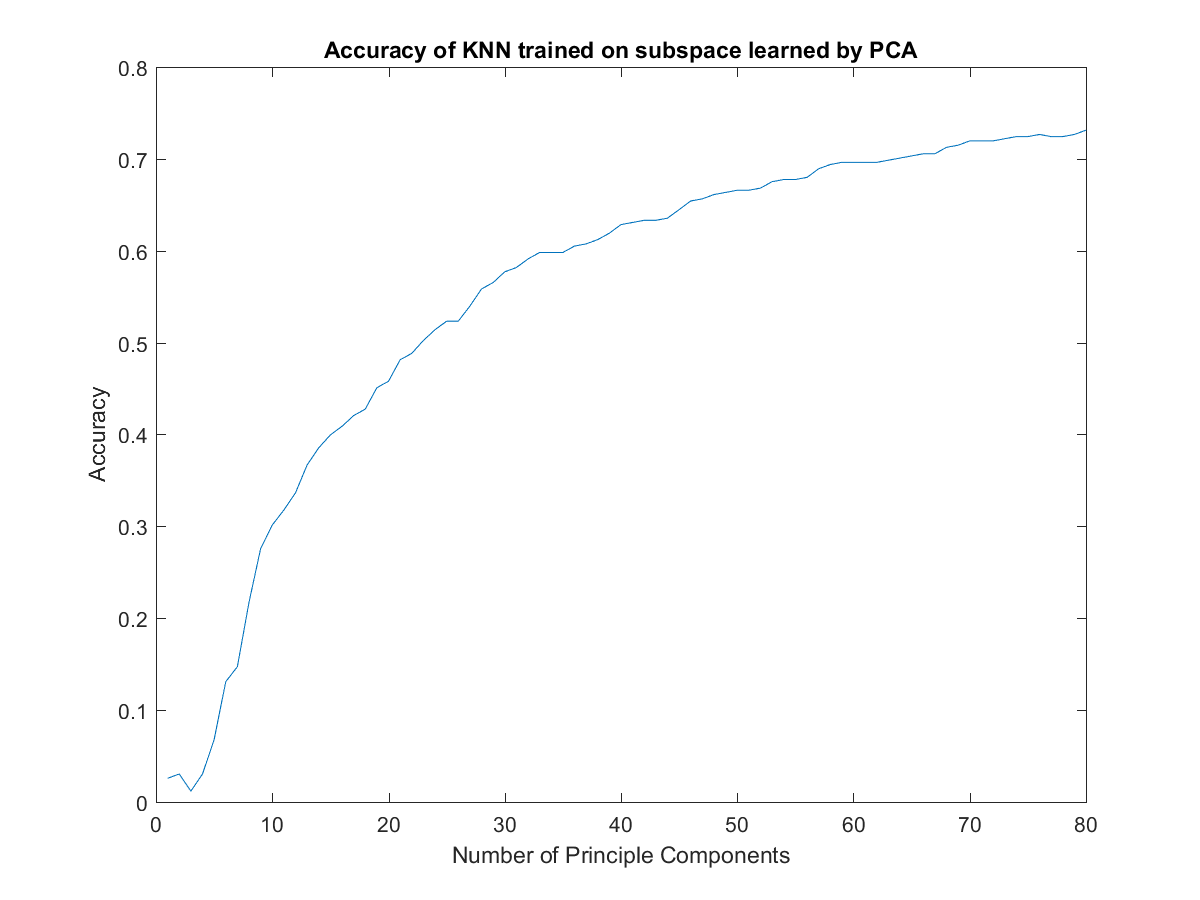
\includegraphics[width = 2in]{figures/cross-val-PCA.png}} &
\subfloat[\fontsize{10}{11}SVD PCA]{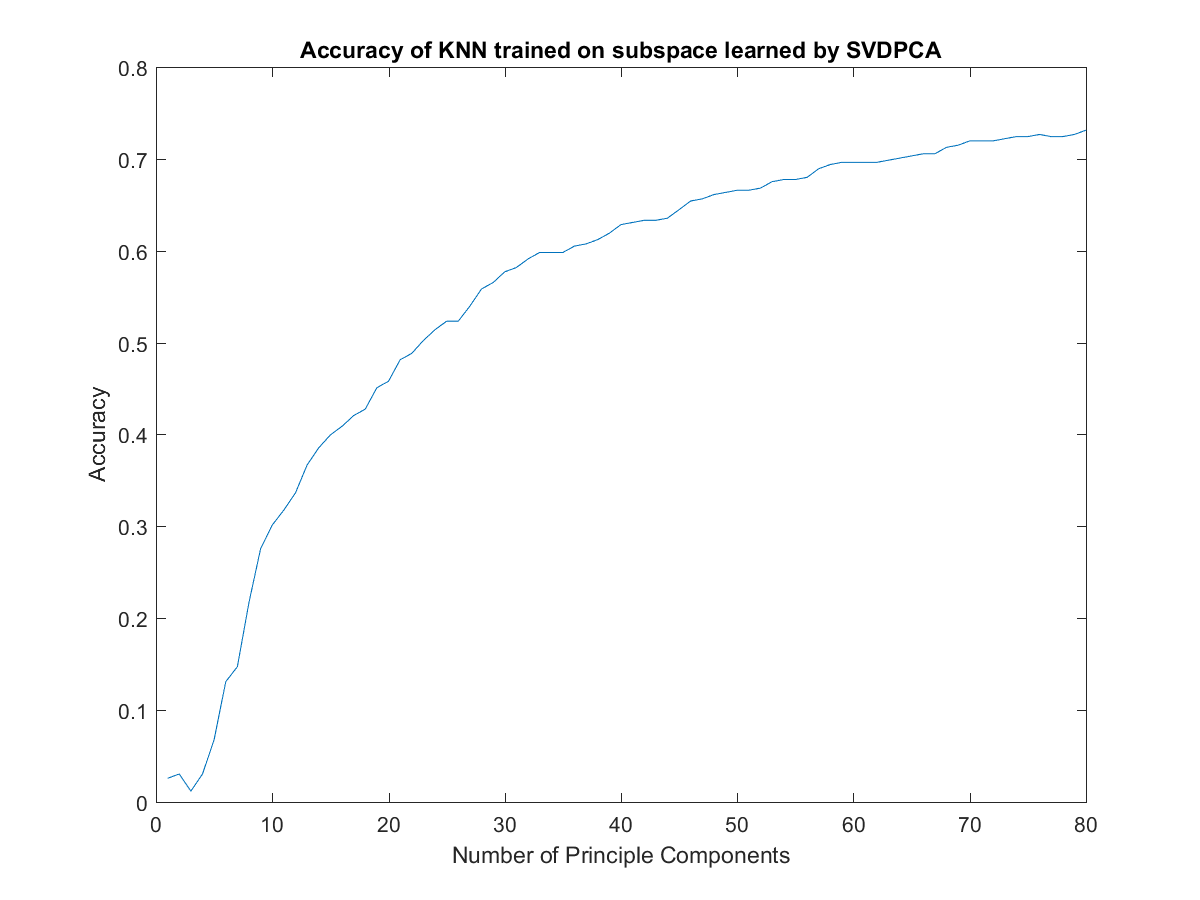
\includegraphics[width = 2in]{figures/cross-val-SVDPCA.png}} &
\subfloat[\fontsize{10}{11}Stochastic Power Method]{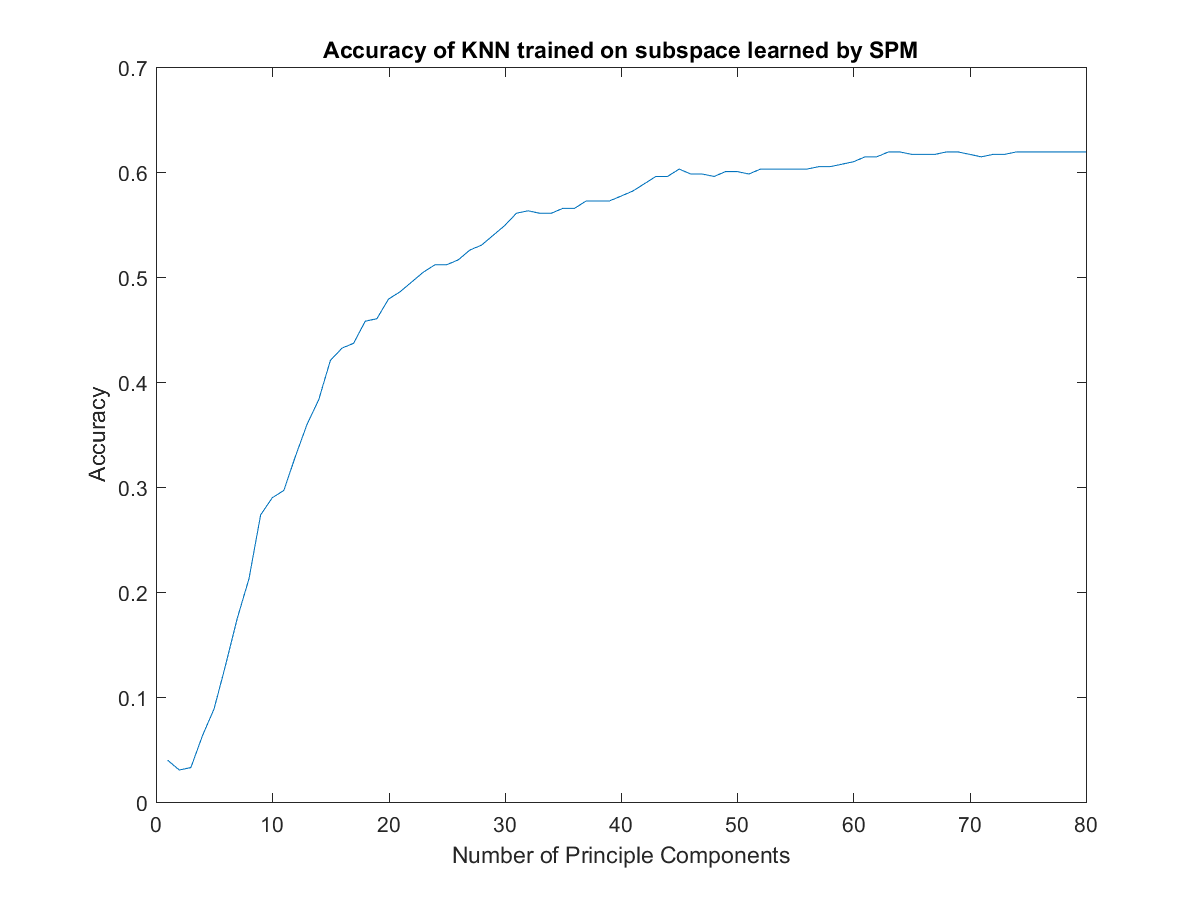
\includegraphics[width = 2in]{figures/cross-val-SPM.png}} \\
\subfloat[\fontsize{10}{11}Incremental PCA]{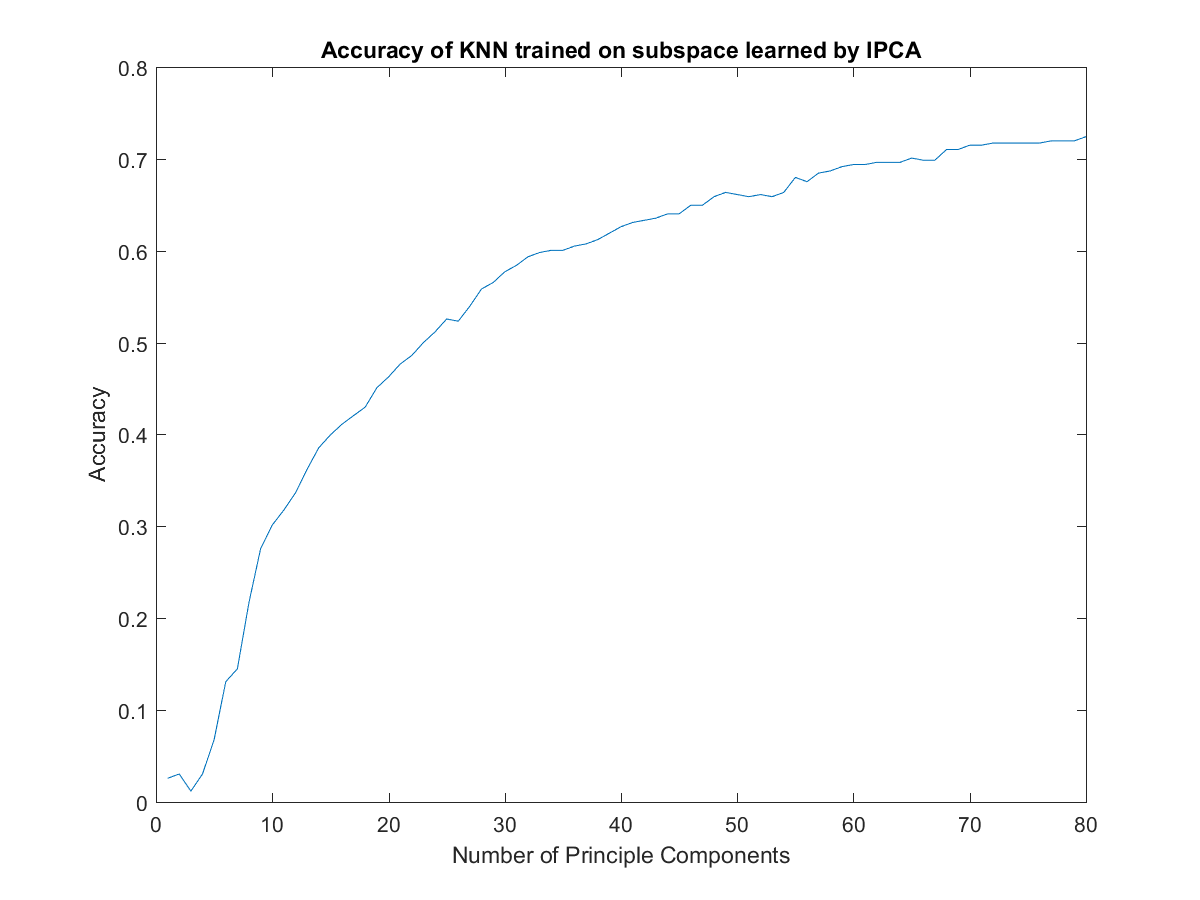
\includegraphics[width = 2in]{figures/cross-val-IPCA.png}} &
\subfloat[\fontsize{10}{11}Matrix Stochastic Gradient]{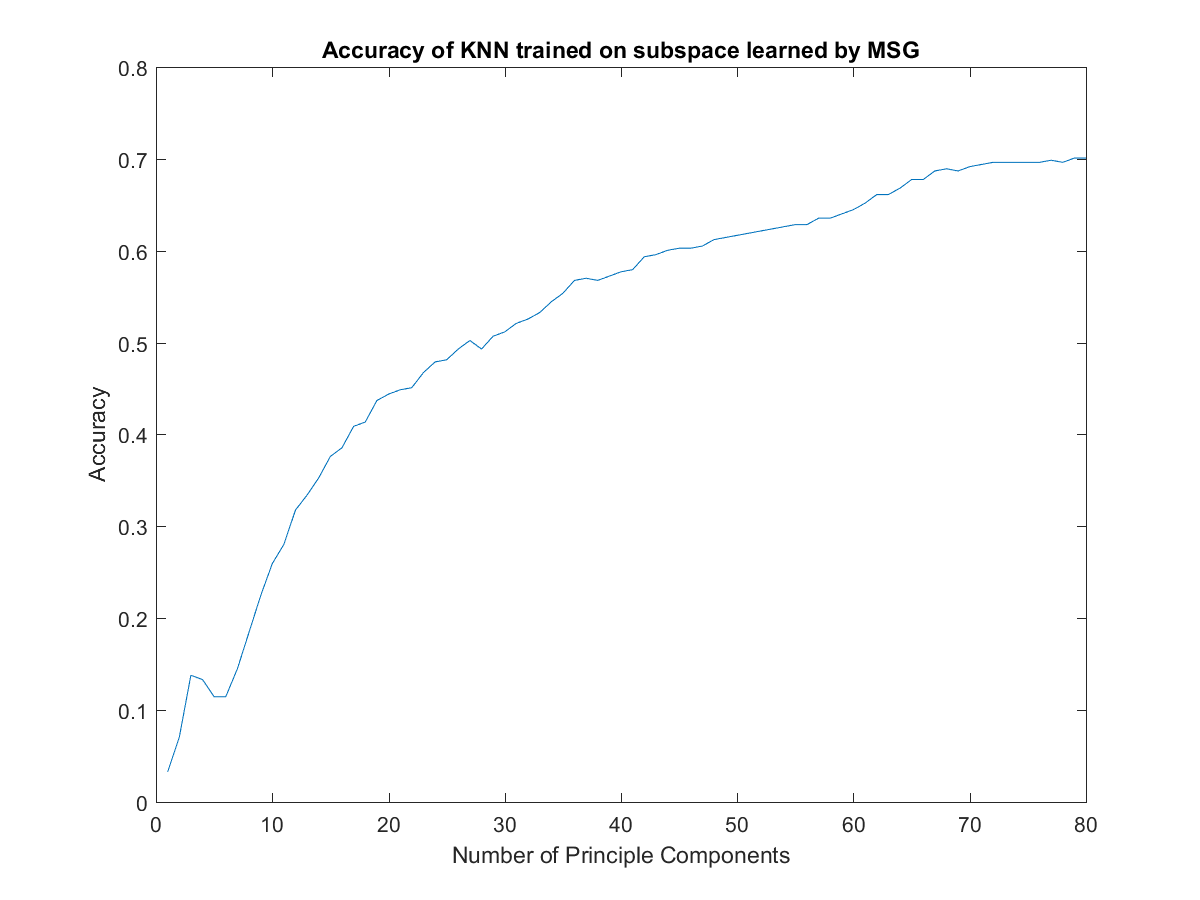
\includegraphics[width = 2in]{figures/cross-val-MSG.png}} &
\subfloat[\fontsize{10}{11}Sparse PCA]{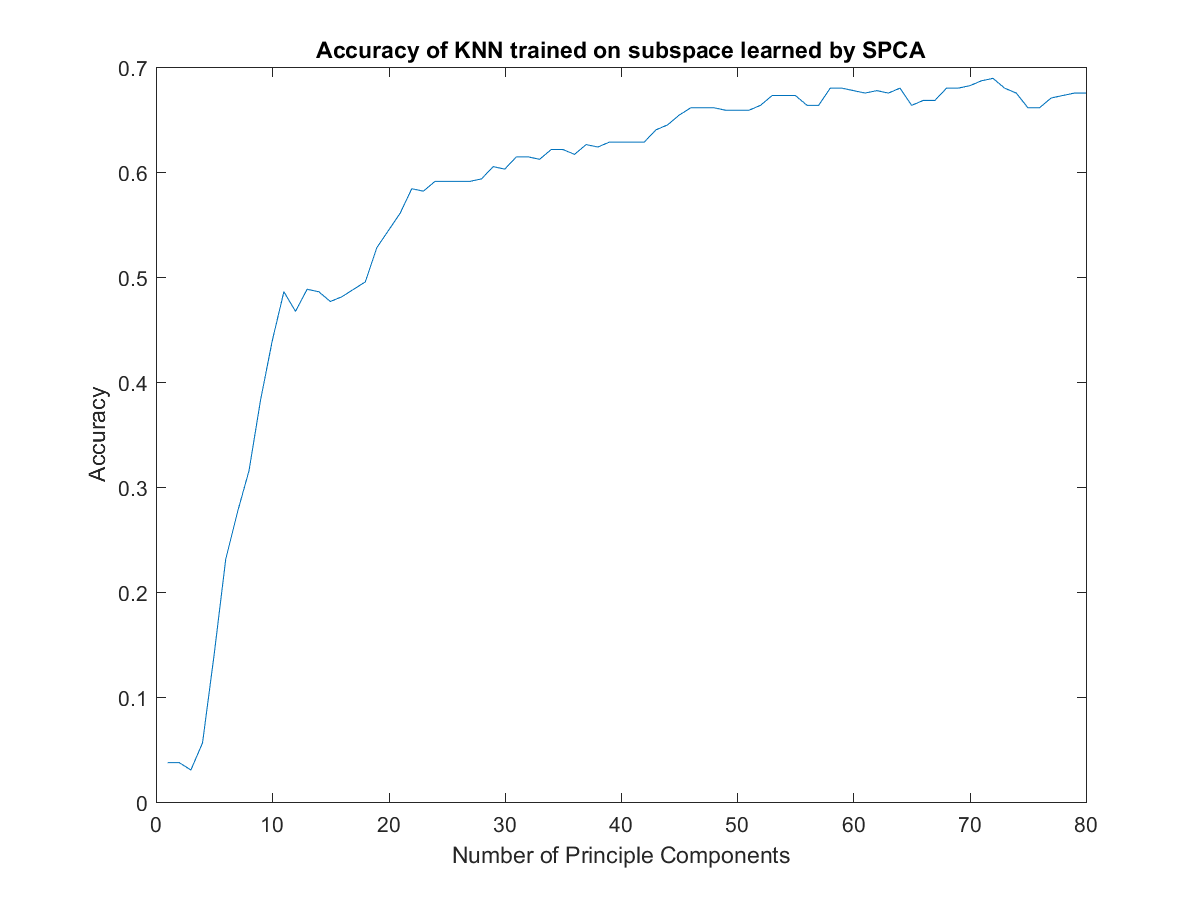
\includegraphics[width = 2in]{figures/cross-val-SPCA.png}} 

\end{tabular}
\caption{\fontsize{10}{11}Percent Accuracy vs Number of Principle Components for each PCA method}
\end{figure*}


\begin{table}
\begin{center}
\begin{tabular}{|l|rl|}
\hline \bf \fontsize{10}{11}Algorithm & \bf Accuracy & \bf Time\\ \hline
\fontsize{10}{11}Matlab PCA & 75\% & 1:00 \\
\fontsize{10}{11}SPM & 63\% & 4:30 \\
\fontsize{10}{11}IPCA & 75\%  &  2:00 \\
\fontsize{10}{11}MSG & 71\%  &   17:20 \\
\fontsize{10}{11}SVD PCA & 75\% & 1:25 \\
\fontsize{10}{11}SPCA & 72\% & 6:51  \\
\fontsize{10}{11}Direct KNN & 83\%  &   - \\

\hline
\end{tabular}
\end{center}
\caption{\label{font-table} Average accuracy achieved by each algorithm and time to convergence (min:sec)}
\end{table}
Figure 1 shows the classification accuracy of each method implemented against the number of principle components used. Table 1 shows the best classification accuracy of each method as well as the overall time it took to train and test K-NN. As expected, the accuracy increases monotonically with the number of principle components, but diminishingly so. 

 We confirm the result of the landmark paper by Turk and Pentland that 40 principle components is sufficient to learn a high fidelity subspace \cite{turk}. However, we did not extend these algorithms to the pattern recognition task of identifying faces in more complex image, nor did we weight the eigenfaces such that each real face could be constructed from a linear combination thereof. We theorize that realtime recognition and detection systems could benefit from the methods discussed in this study because globalization has made international travel more accessible, making the streaming model of computation more relevant. 

The Matlab built-in PCA, SVD PCA\footnote{This is simply direct computation of the subspace by observing that the covariance matrix $XX^{\top} = US^2U^\top$ for $X = USV^\top$}, and Incremental PCA achieved the best accuracy overall with 75\% accuracy with the fastest convergence. Sparse PCA does reasonable well with 72\% accuracy, compared to the other methods. Interestingly, sparse PCA immediately finds a few very expressive principle componts. Matrix stochastic gradient is by far the slowest to converge, but again enjoys better theoretical guarantees. Stochastic power method is much more sensitive to its learning rate, and performing a more fine tuned grid search over $\eta$ was outside our time constraints. However, all of these algorithms should learn the same subspace to within small rotations and scalings. 

One limitation to this dataset is its small sample size (only $\approx$ 2000 images in total) and even smaller label set (only 38 individuals). These algorithms are intended to be applied to orders of magnitude larger datasets. 

Figure 2 shows the original face used in reconstruction. Figure 5 shows the examples of that face reconstructed using only the top five principle components for the corresponding algorithm. Figure 6 shows the original face reconstructed faces with 30 principle components.

Figure 3 shows an example of the ``eigenfaces'' of the first principle components for each algorithm, Figure 4 shows the thresholded ``eigenfaces'' of the same principle components.   To our surprise, the top eigenfaces captured the effects of the lighting conditions (rather than eyes, nose, or chin, it learned the right or left half of faces). Eyebrows, pupils, lips, and cheekbones were also points of focus. 


From looking at both the reconstruction and ``eigenfaces'' we see some explanation for the data. Incremental PCA, SVD PCA, and the Matlab PCA all learn similar ``eigenfaces'' and focus on similar anatomical details. Sparse PCA, paradoxically, is more difficult to interpret. 

Figure 7 shows the variance captured by the corresponding number of principle components. For the overall data, after centering and normalization, the variance was approximately $3.55 e^7$. These match the accuracy result earlier, with SVD PCA and incremental PCA capturing the most variance. Interestingly though, sparse PCA captures less variance than the stochastic power method, but still manages to outperform in terms of accuracy. Most users select $k$ such that some threshold of the data variance is captured by the subspace.

\begin{figure}
\center
\subfloat{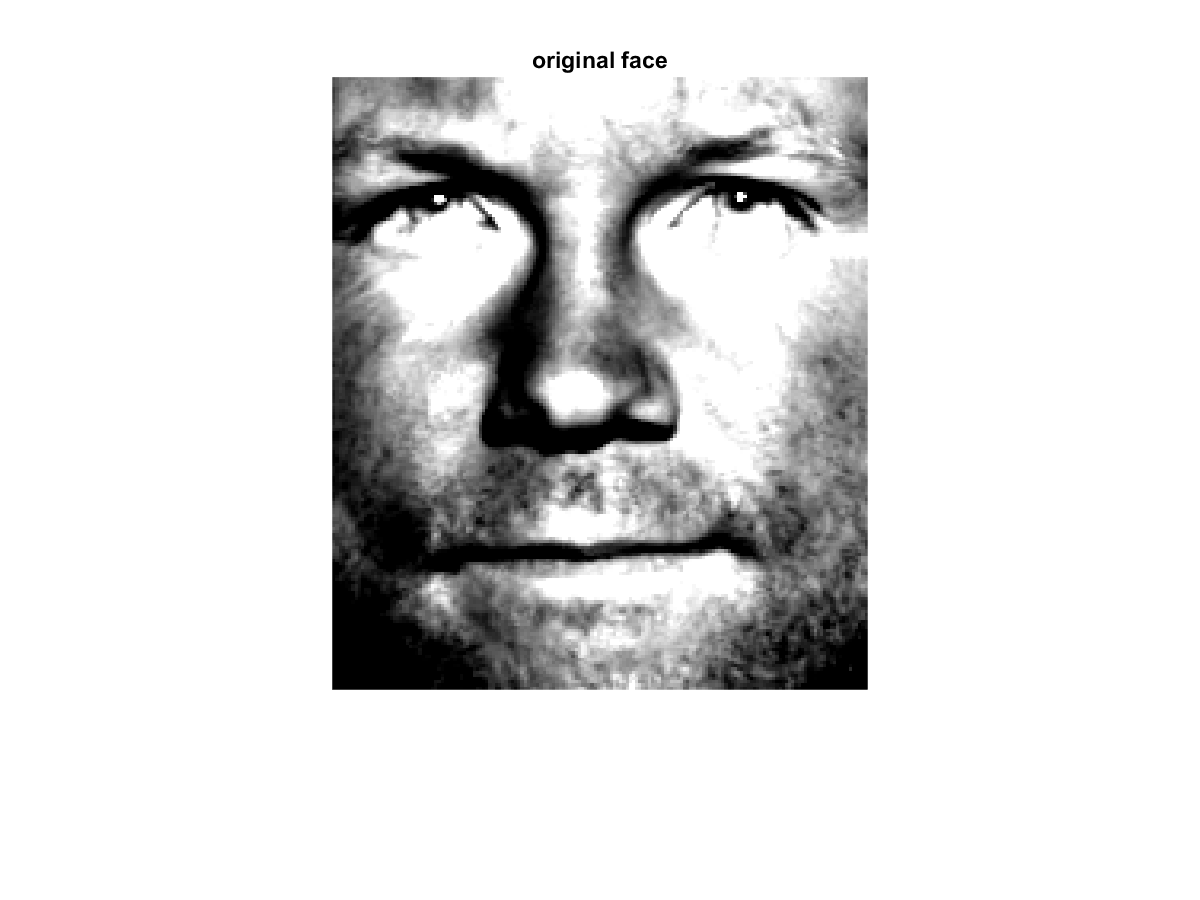
\includegraphics[width = 2in]{figures/PCA-Faces/original face}}
\caption{\fontsize{10}{11} Original Face used for Reconstruction}
\end{figure}

\begin{figure*}[H]
\begin{tabular}{ccc}
\subfloat[\fontsize{10}{11} Matlab ]{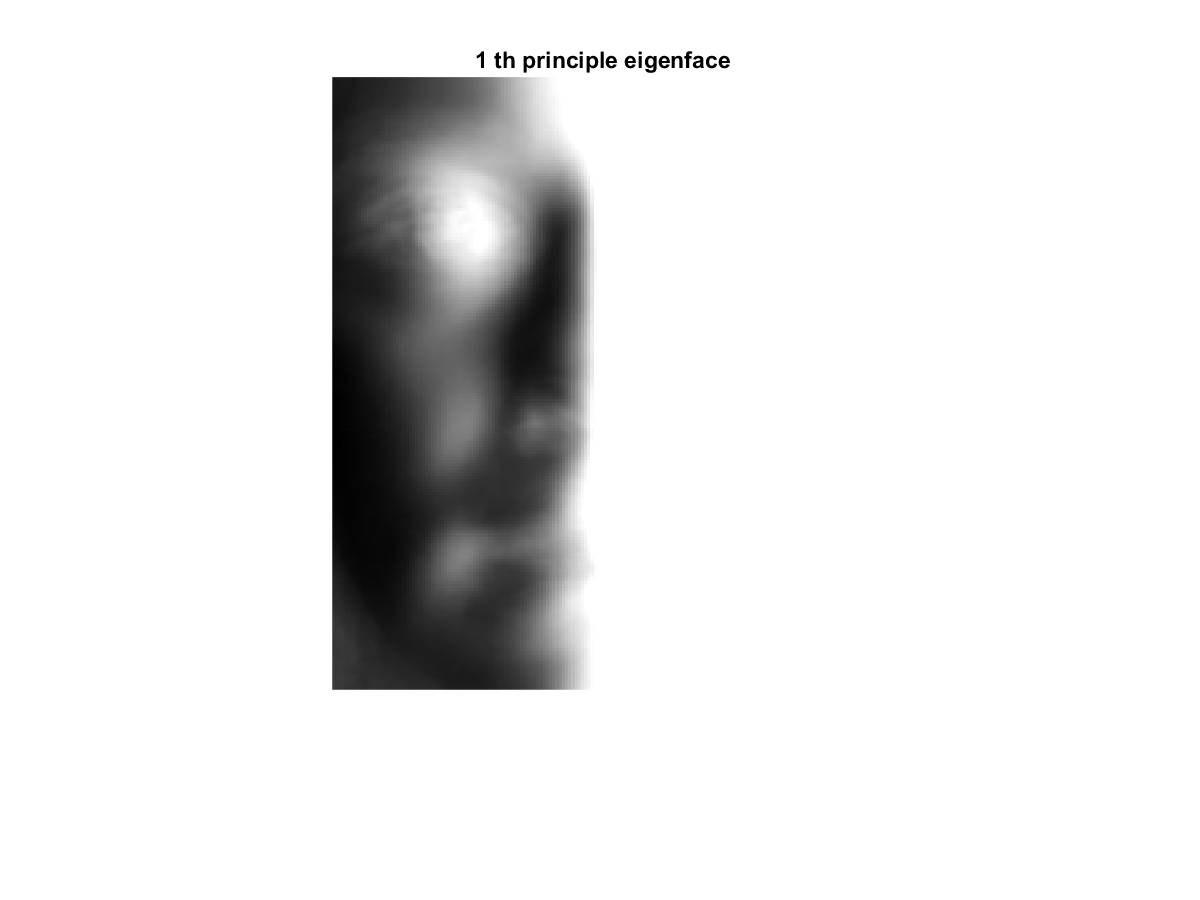
\includegraphics[width = 2in]{figures/PCA-Faces/eigenface_number_1.png}} &
\subfloat[\fontsize{10}{11} SPM]{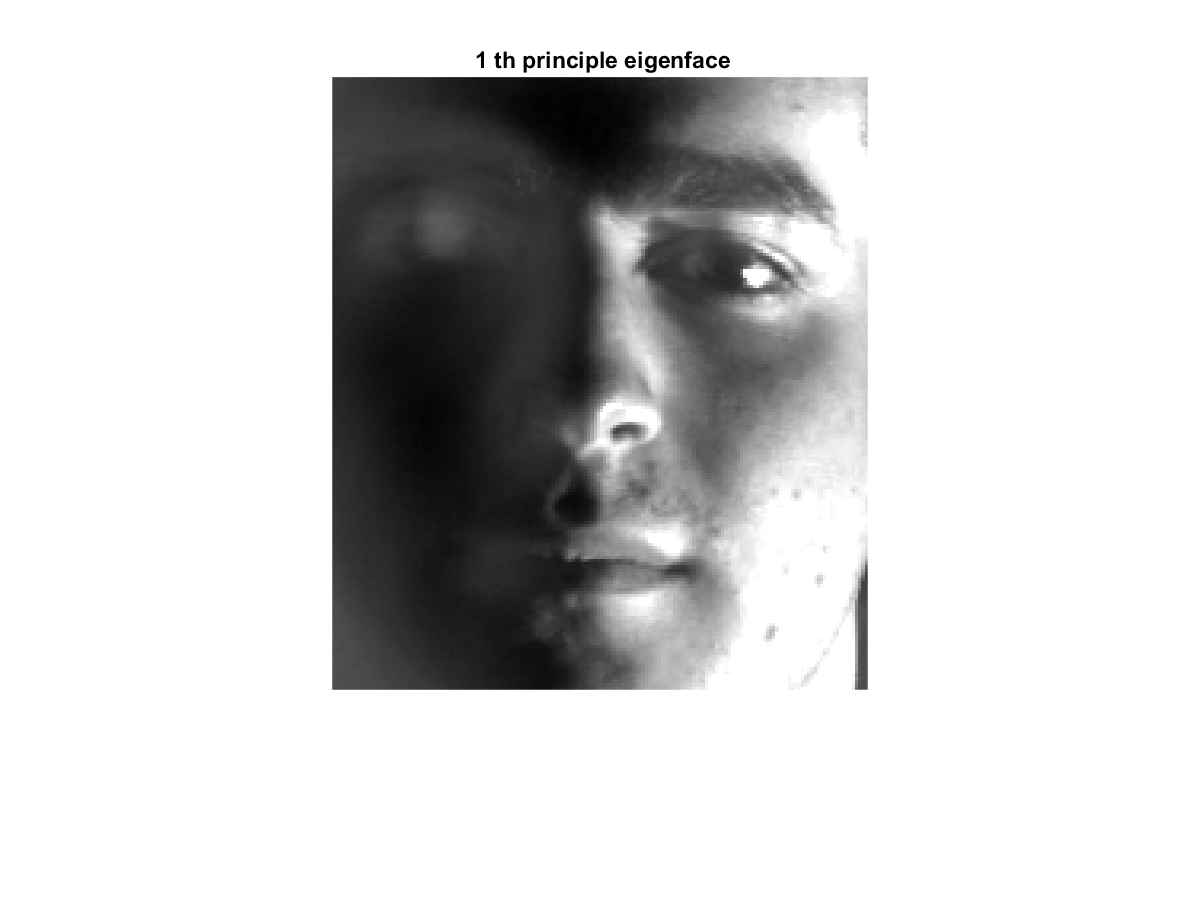
\includegraphics[width = 2in]{figures/SPM-Faces/eigenface_number_1.png}} &
\subfloat[\fontsize{10}{11} IPCA ]{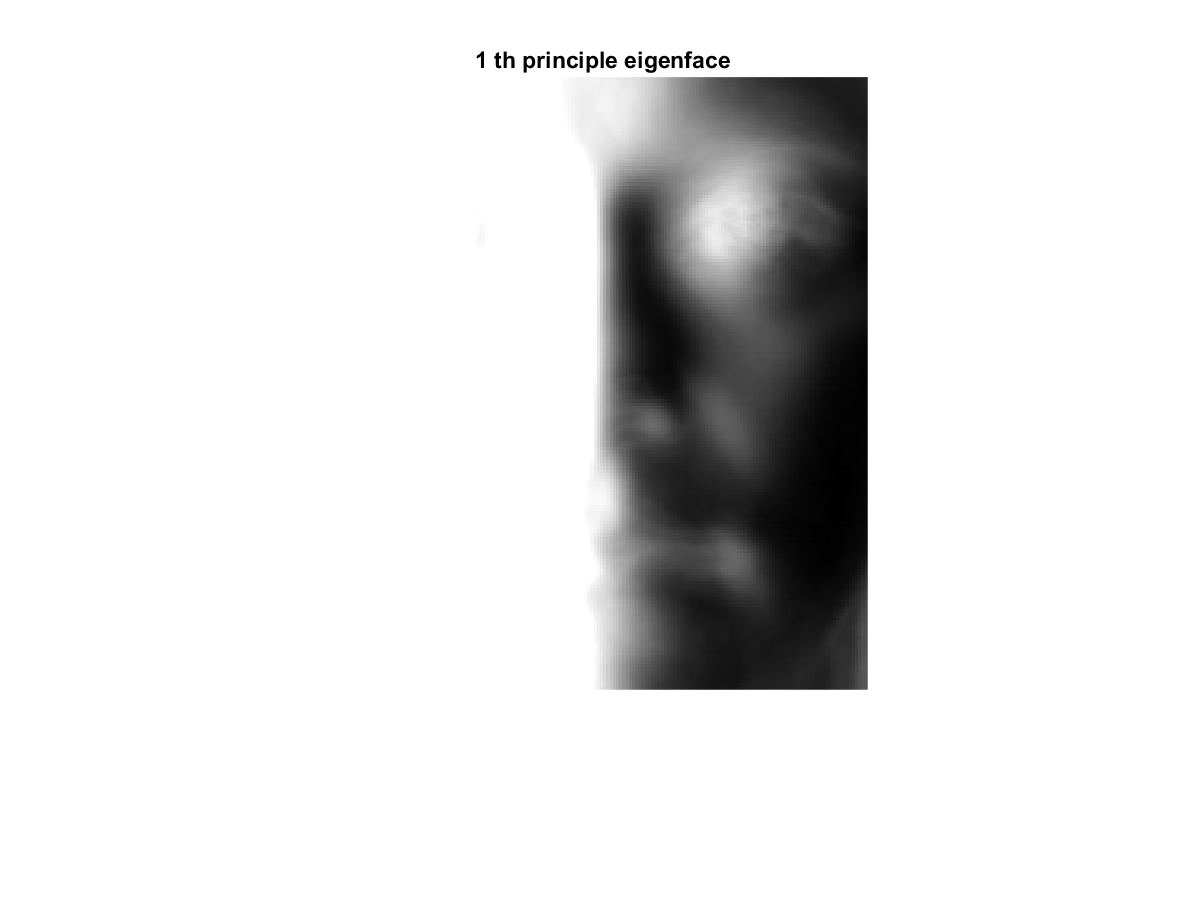
\includegraphics[width = 2in]{figures/IPCA-Faces/eigenface_number_1.png}} \\
\subfloat[\fontsize{10}{11} MSG ]{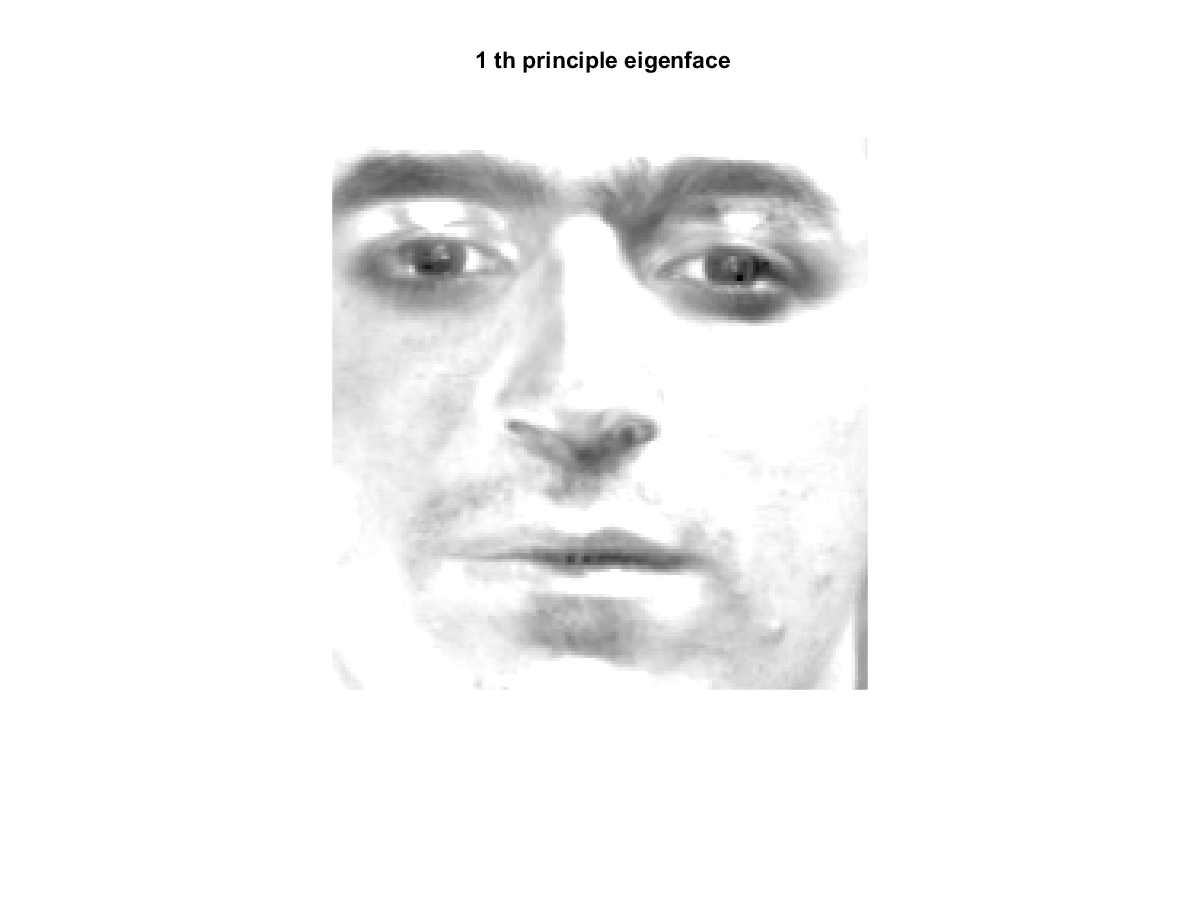
\includegraphics[width = 2in]{figures/MSG-Faces/eigenface_number_1.png}} &
\subfloat[\fontsize{10}{11} SVD PCA ]{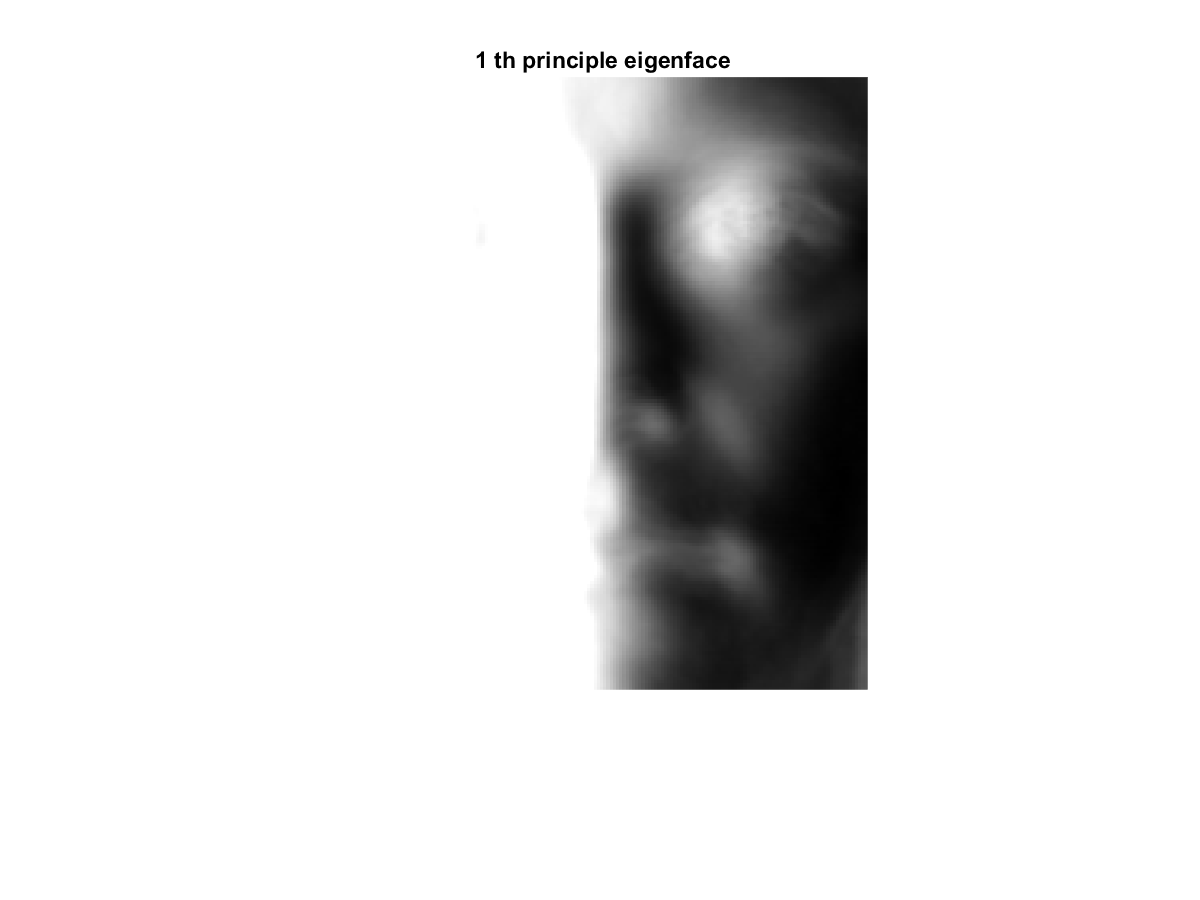
\includegraphics[width = 2in]{figures/SVDPCA-Faces/eigenface_number_1.png}} &
\subfloat[\fontsize{10}{11} SPCA ]{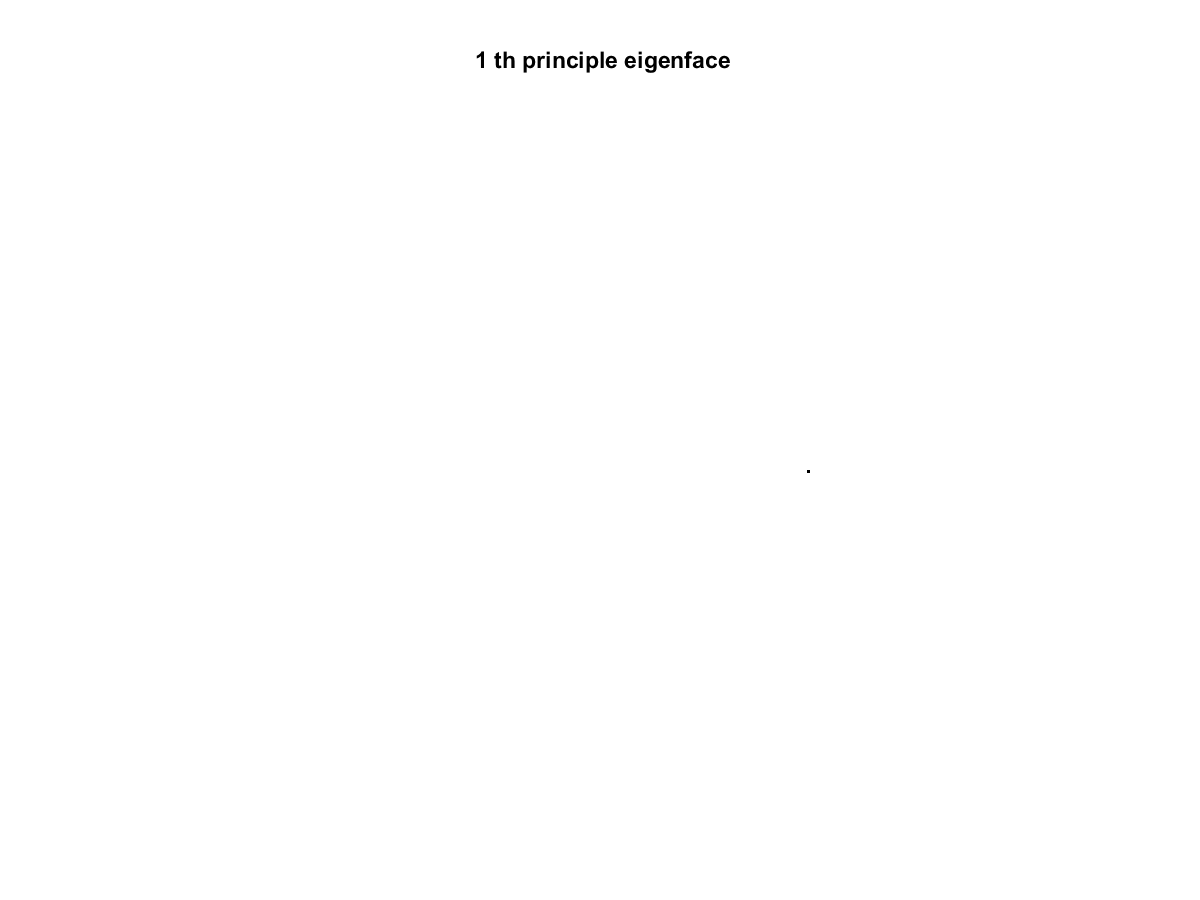
\includegraphics[width = 2in]{figures/SPCA-Faces/eigenface_number_1.png}}  

\end{tabular}
\caption{\fontsize{10}{11} Examples of ``Eigenfaces''}
\end{figure*}


\begin{figure*}[ht]
\begin{tabular}{ccc}
\subfloat[\fontsize{10}{11} Matlab ]{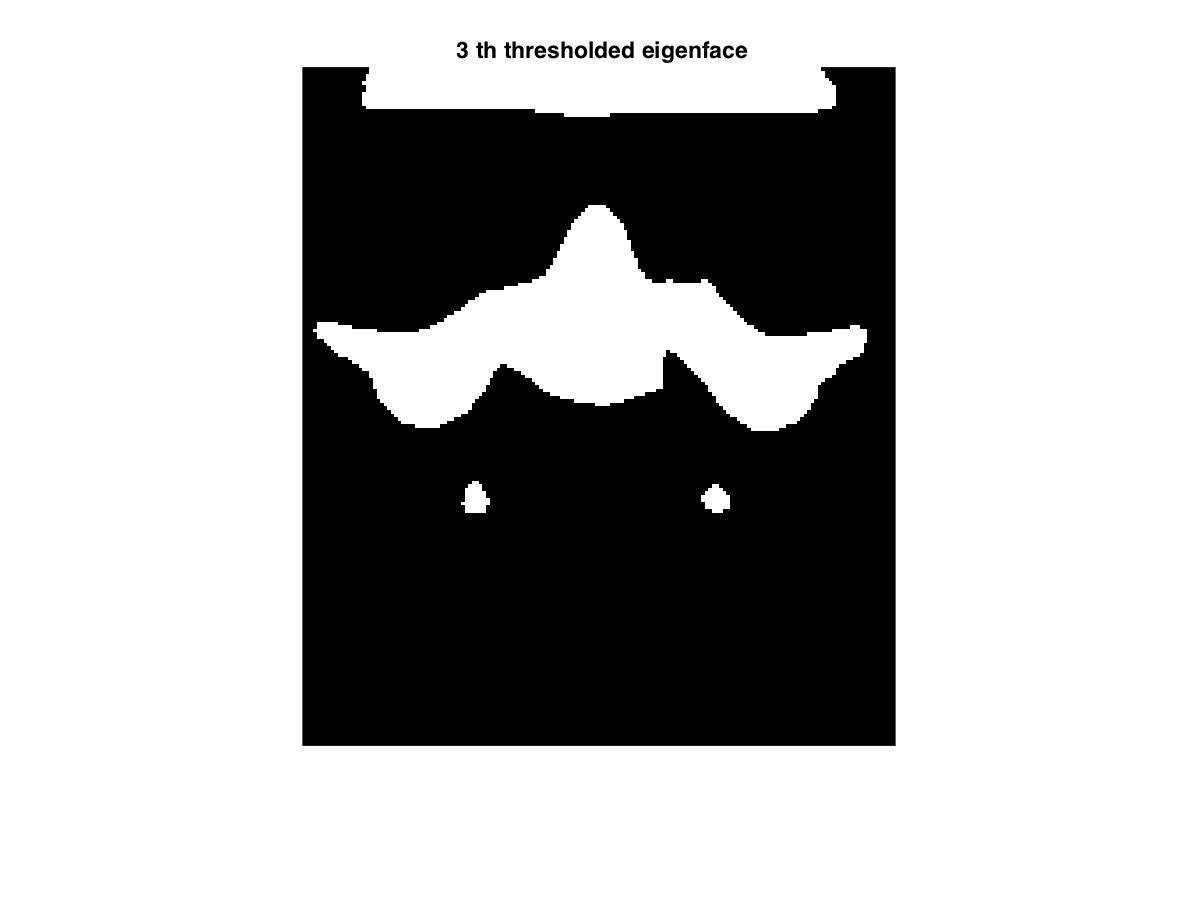
\includegraphics[width = 2in]{figures/PCA-Faces/thresholded_eigenface_number_3.png}} &
\subfloat[\fontsize{10}{11} SPM]{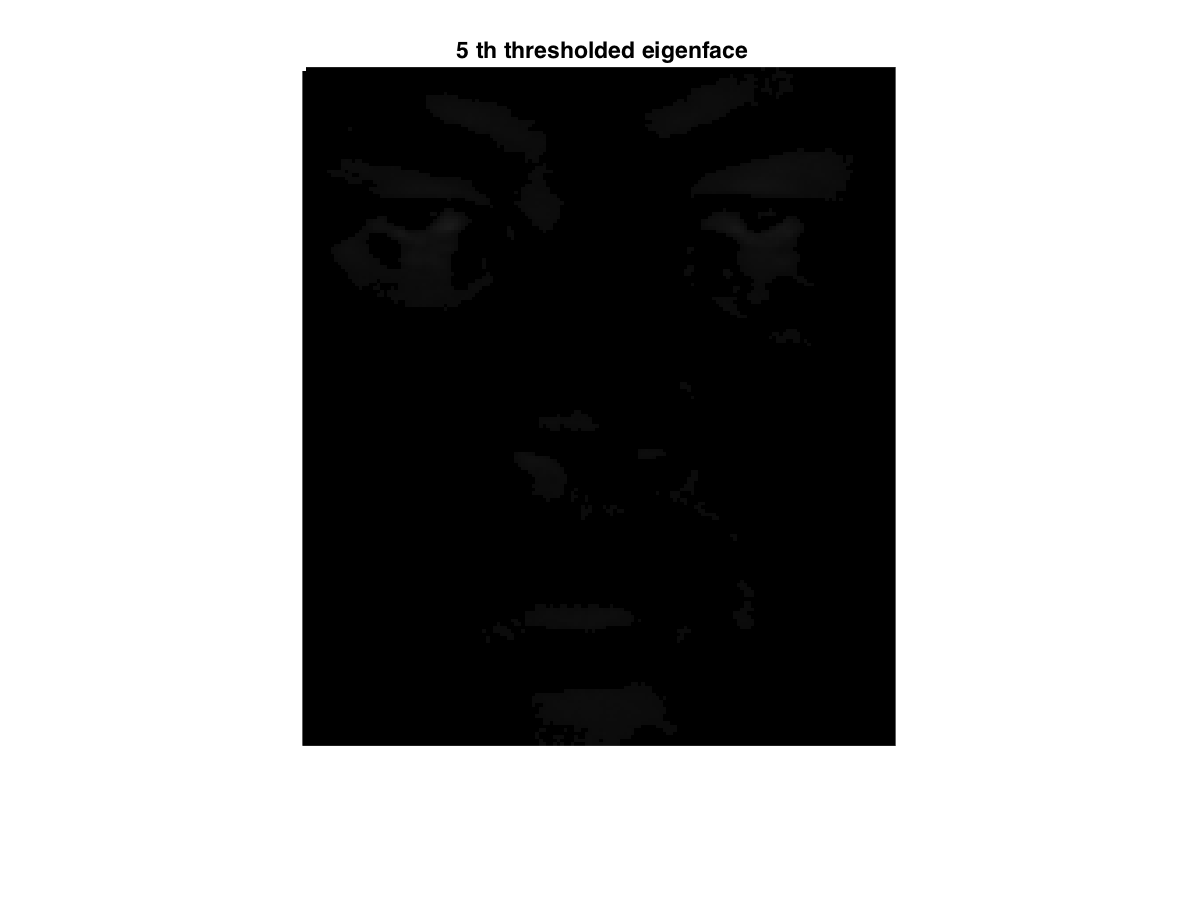
\includegraphics[width = 2in]{figures/SPM-Faces/thresholded_eigenface_number_5.png}} &
\subfloat[\fontsize{10}{11} IPCA ]{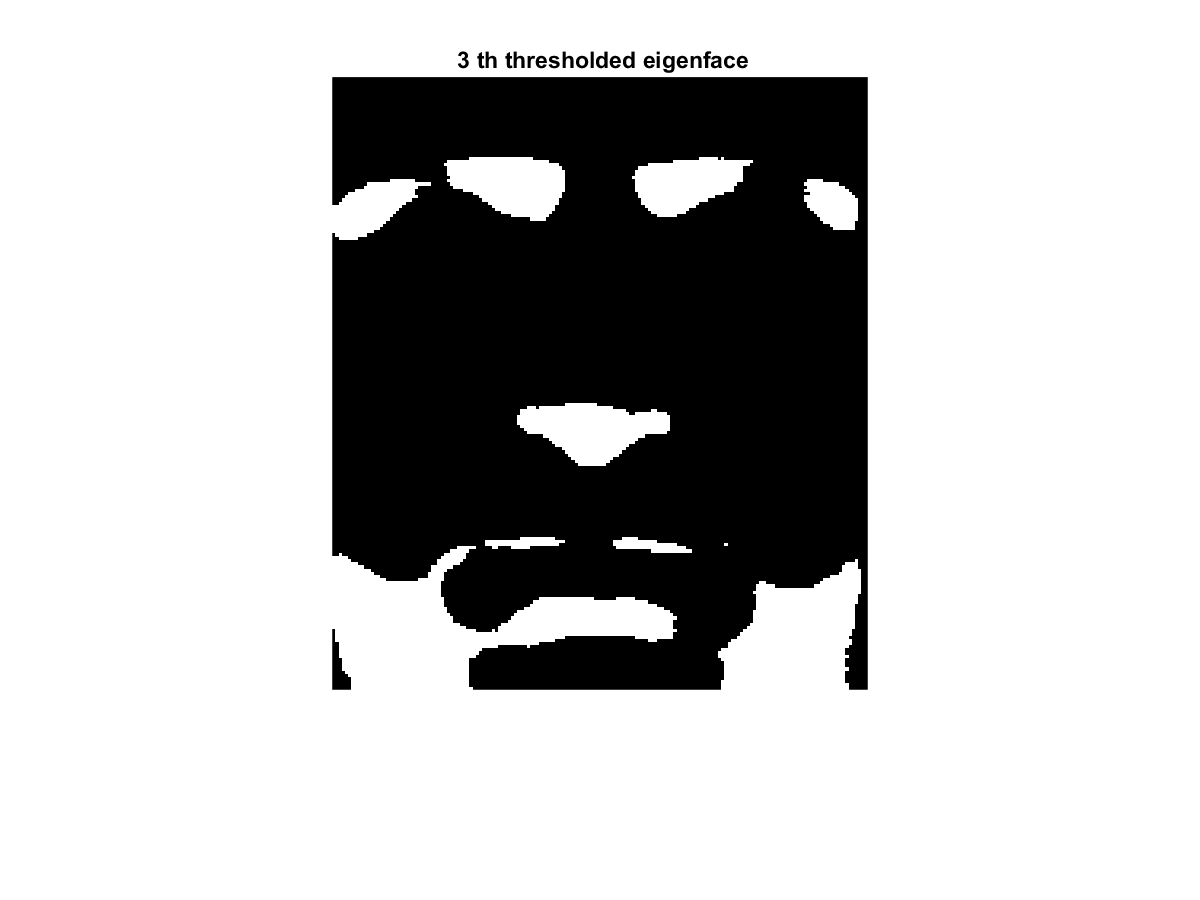
\includegraphics[width = 2in]{figures/IPCA-Faces/thresholded_eigenface_number_3.png}} \\
\subfloat[\fontsize{10}{11} MSG ]{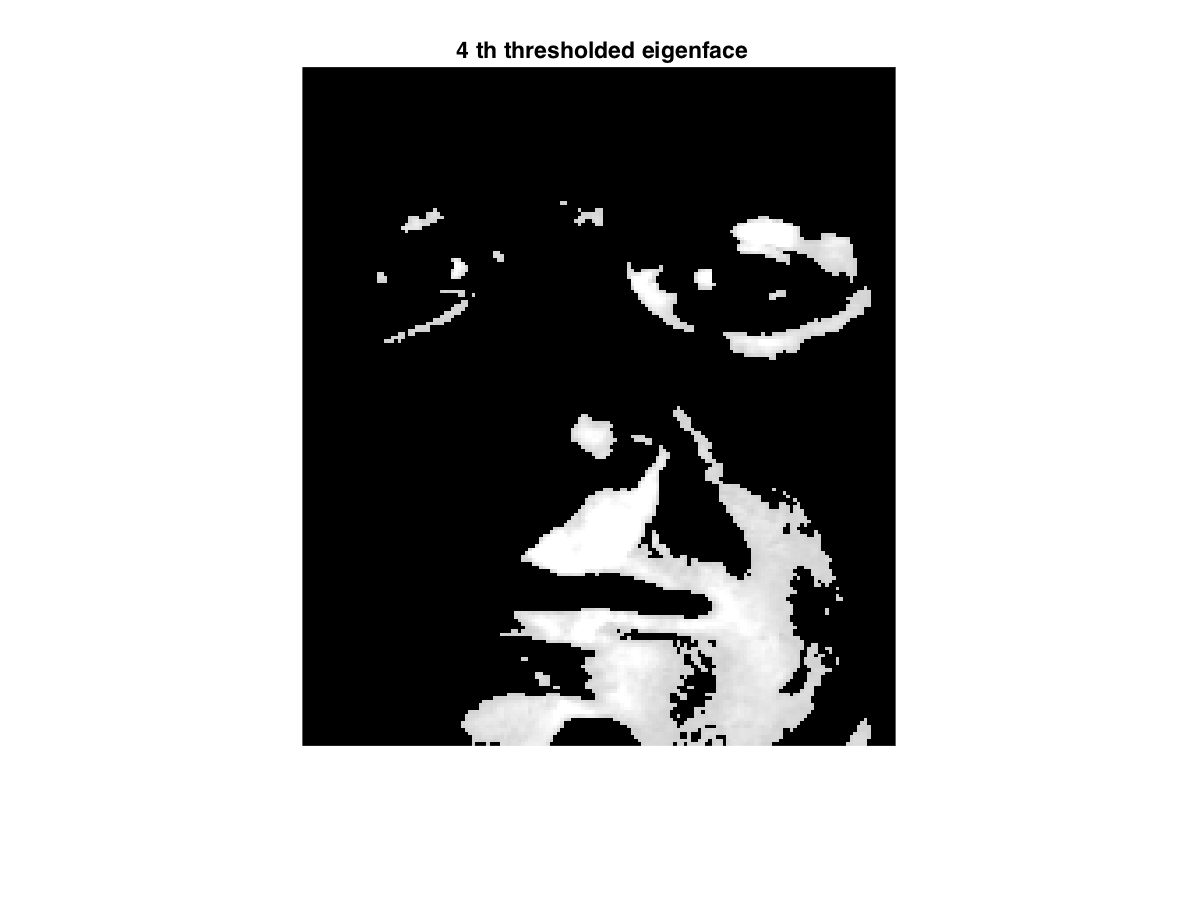
\includegraphics[width = 2in]{figures/MSG-Faces/thresholded_eigenface_number_4.png}} &
\subfloat[\fontsize{10}{11} SVD PCA ]{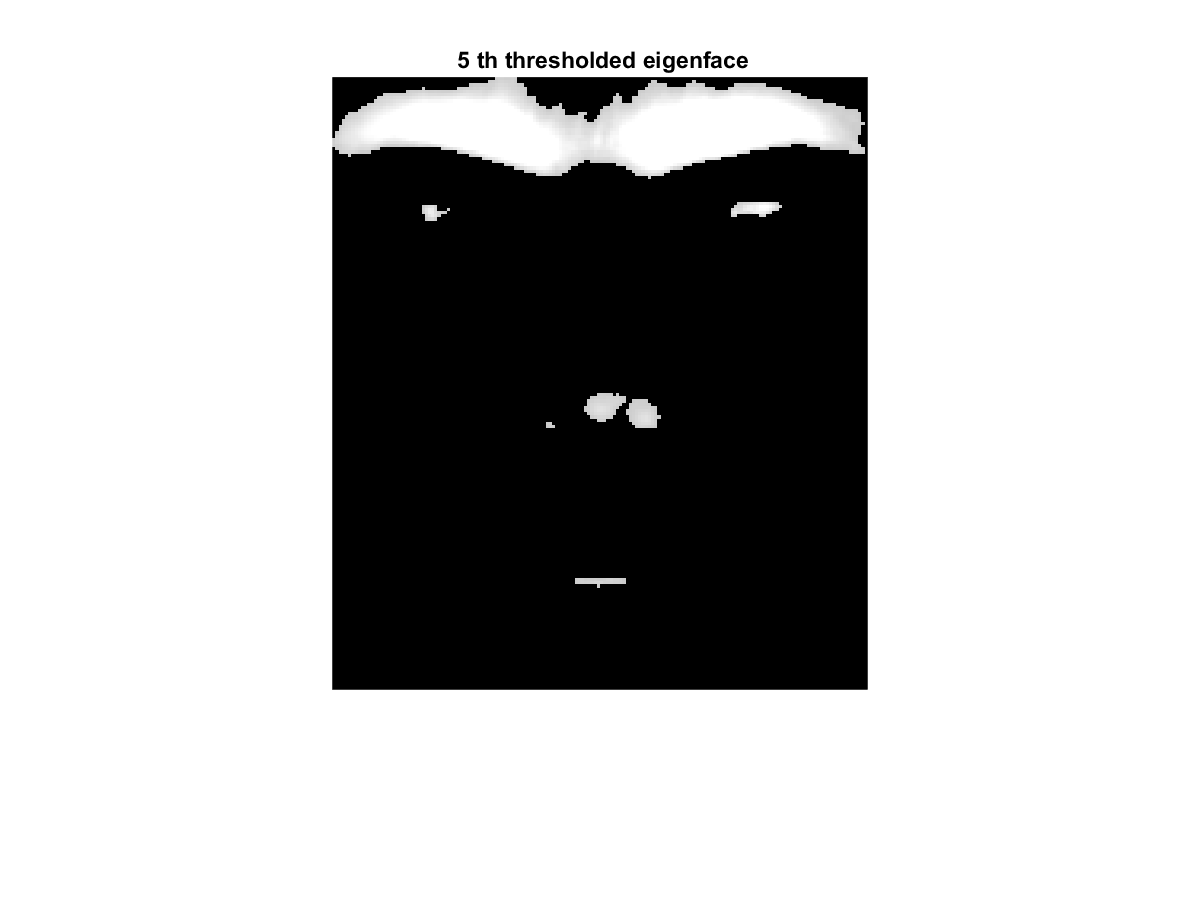
\includegraphics[width =2in]{figures/SVDPCA-Faces/thresholded_eigenface_number_5.png}} &
\subfloat[\fontsize{10}{11} SPCA ]{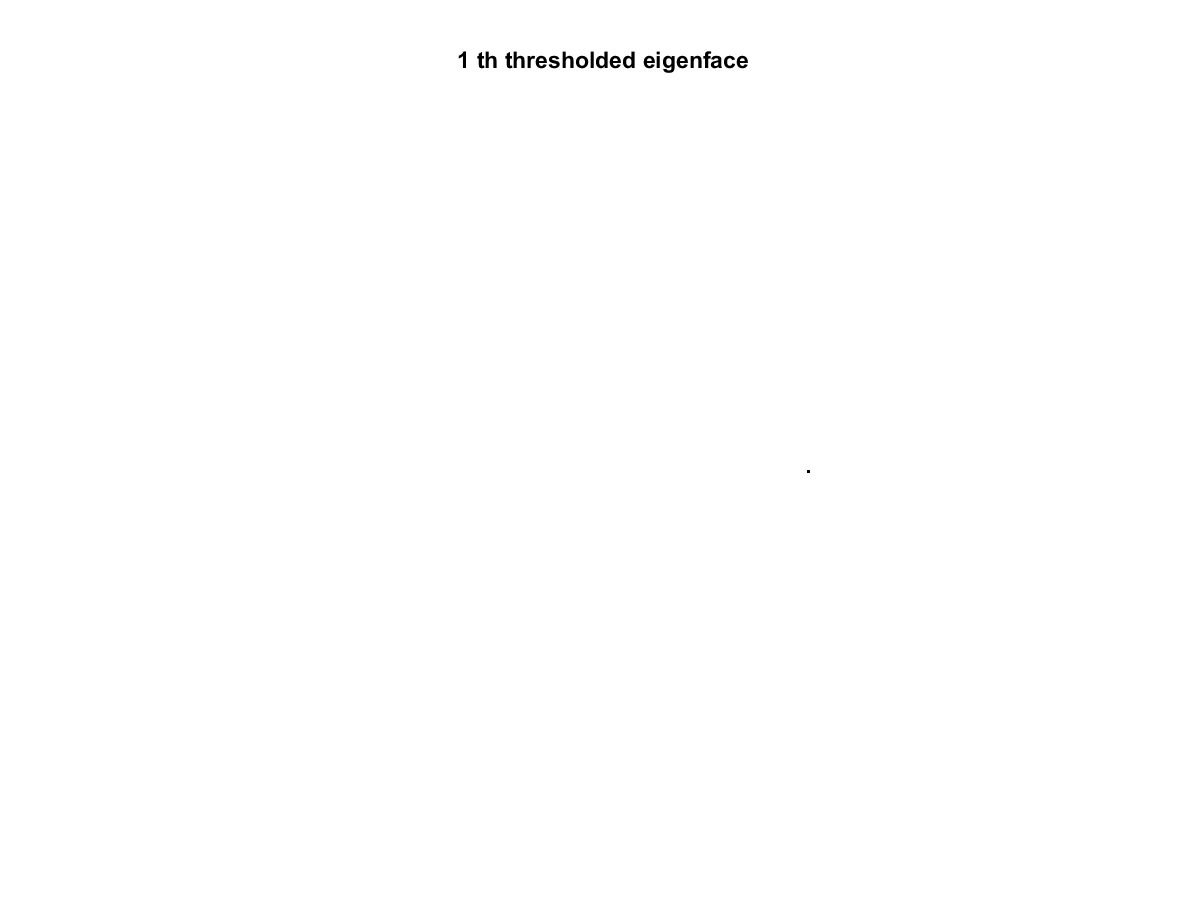
\includegraphics[width = 2in]{figures/SPCA-Faces/thresholded_eigenface_number_1.png}}  

\end{tabular}
\caption{\fontsize{10}{11} Some examples of thresholded ``Eigenfaces'' chosen from among the top 5 principle components. IPCA, built-in PCA, and SVD PCA focus most cleanly on anatomical features (even capturing beauty marks above the lips!), they also achieve the highest accuracy}
\end{figure*}


\begin{figure*}[ht]
\begin{tabular}{ccc}
\subfloat[\fontsize{10}{11} Matlab ]{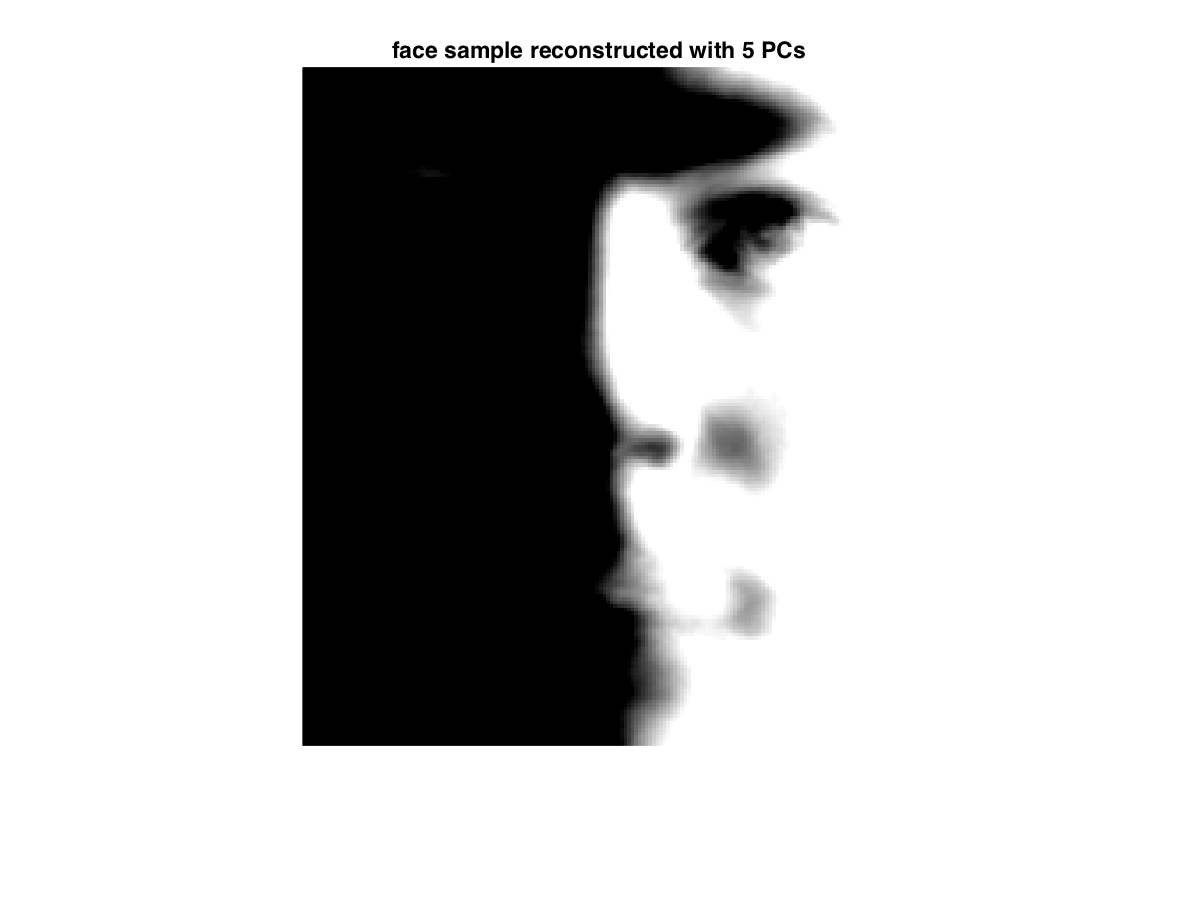
\includegraphics[width = 2in]{figures/PCA-Faces/face sample reconstructed with 5 PCs.png}} &
\subfloat[\fontsize{10}{11} SPM]{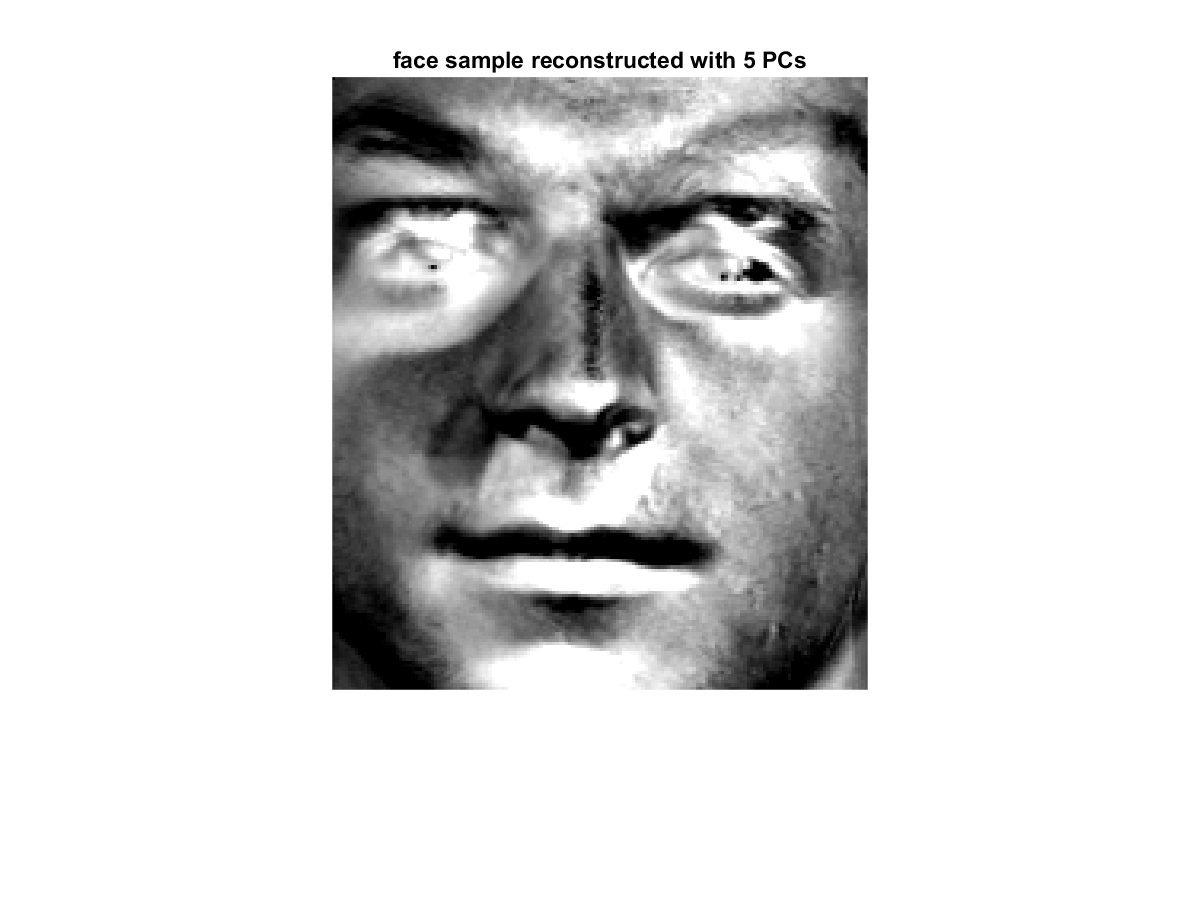
\includegraphics[width = 2in]{figures/SPM-Faces/face sample reconstructed with 5 PCs.png}} &
\subfloat[\fontsize{10}{11} IPCA ]{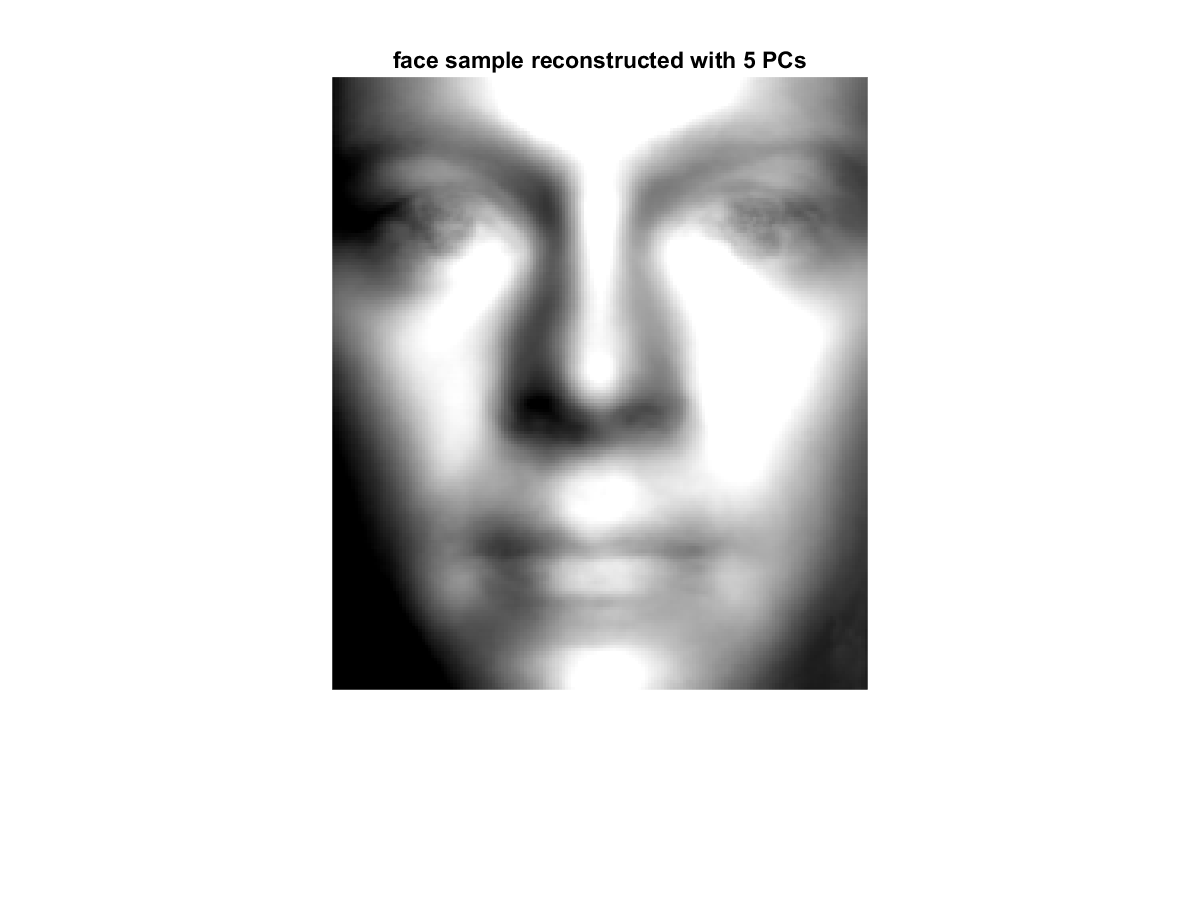
\includegraphics[width = 2in]{figures/IPCA-Faces/face sample reconstructed with 5 PCs.png}} \\
\subfloat[\fontsize{10}{11} MSG ]{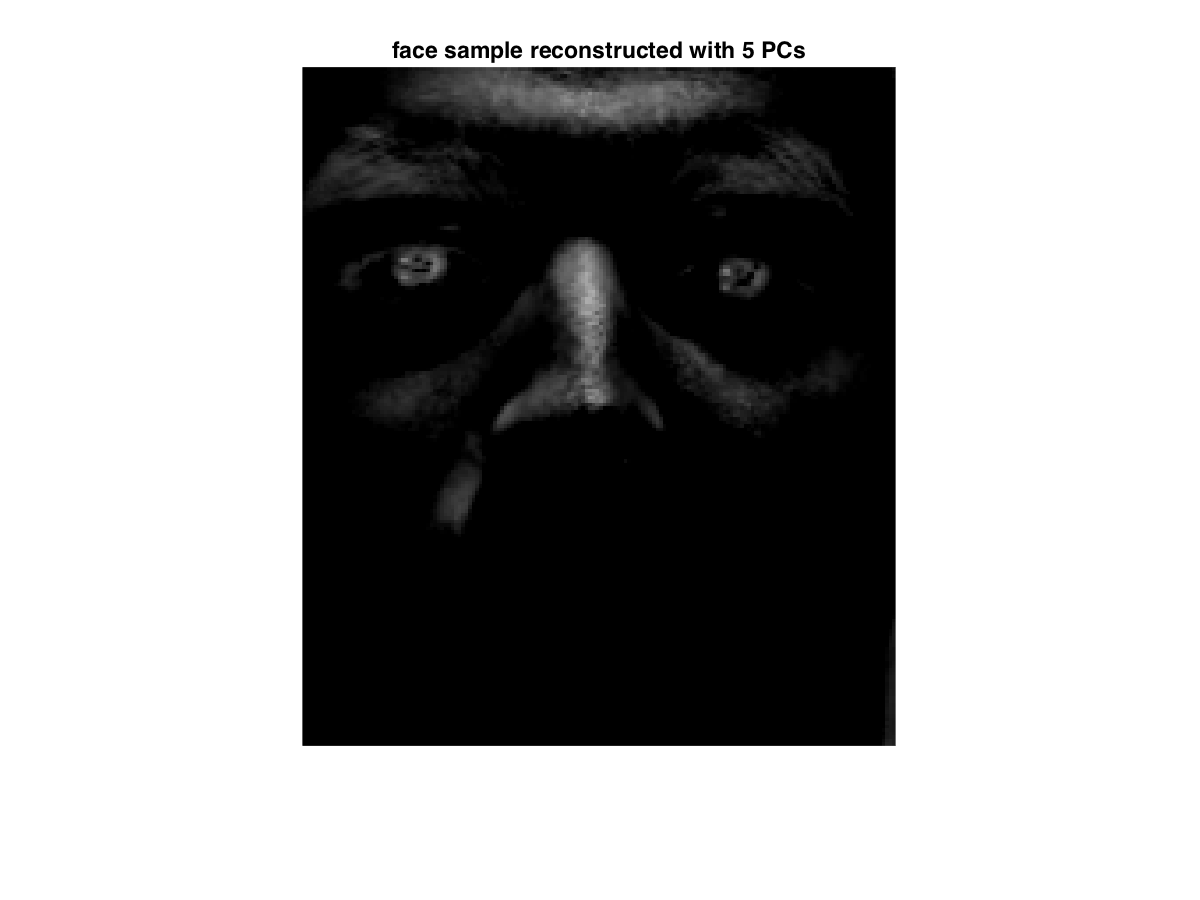
\includegraphics[width = 2in]{figures/MSG-Faces/face sample reconstructed with 5 PCs.png}} &
\subfloat[\fontsize{10}{11} SVD PCA ]{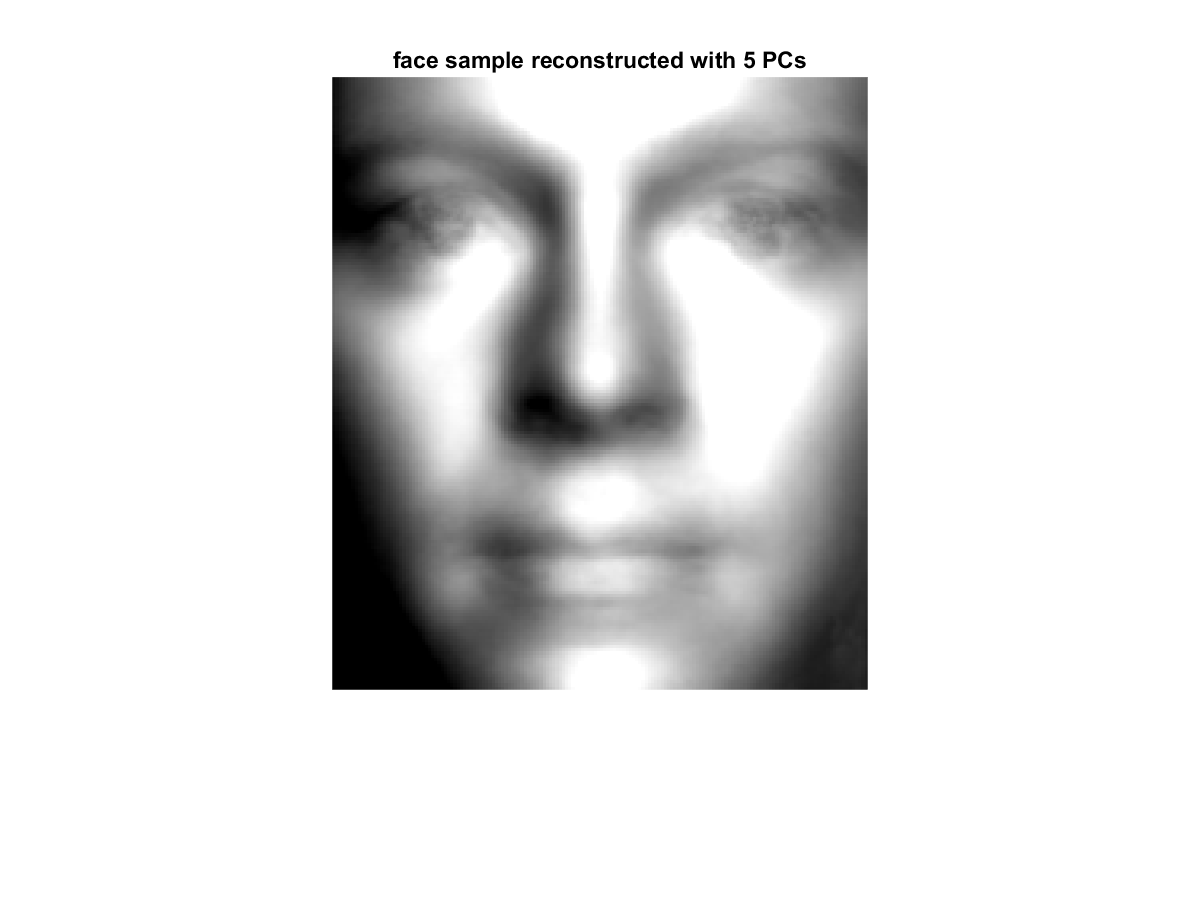
\includegraphics[width =2in]{figures/SVDPCA-Faces/face sample reconstructed with 5 PCs.png}} &
\subfloat[\fontsize{10}{11} SPCA ]{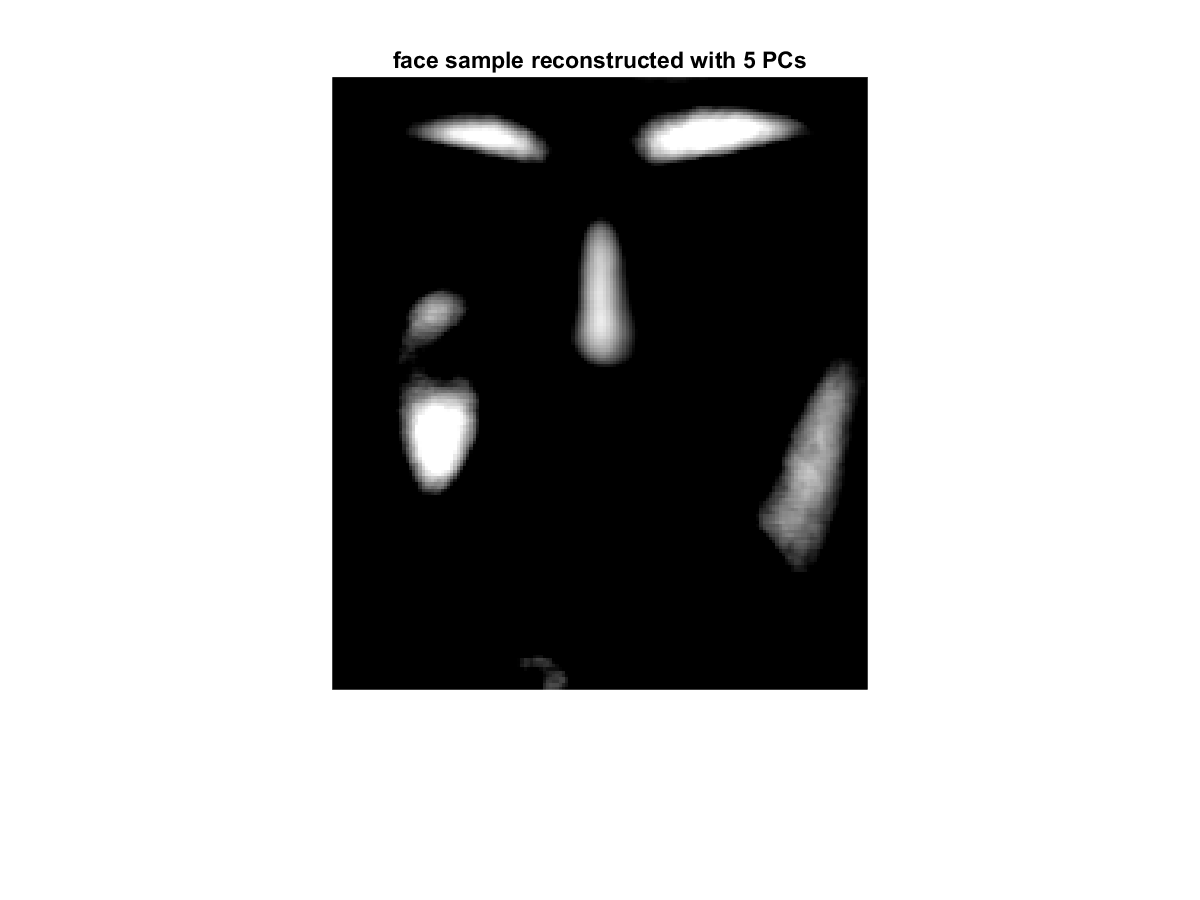
\includegraphics[width = 2in]{figures/SPCA-Faces/face sample reconstructed with 5 PCs.png}}  \\

\end{tabular}
\caption{\fontsize{10}{11} Reconstructed face with 5 Principle Components}
\end{figure*}

\begin{figure*}[ht]
\begin{tabular}{ccc}
\subfloat[\fontsize{10}{11} Matlab ]{\includegraphics[width = 2in]{figures/PCA-Faces/face sample reconstructed with 30 PCs.png}} &
\subfloat[\fontsize{10}{11} SPM]{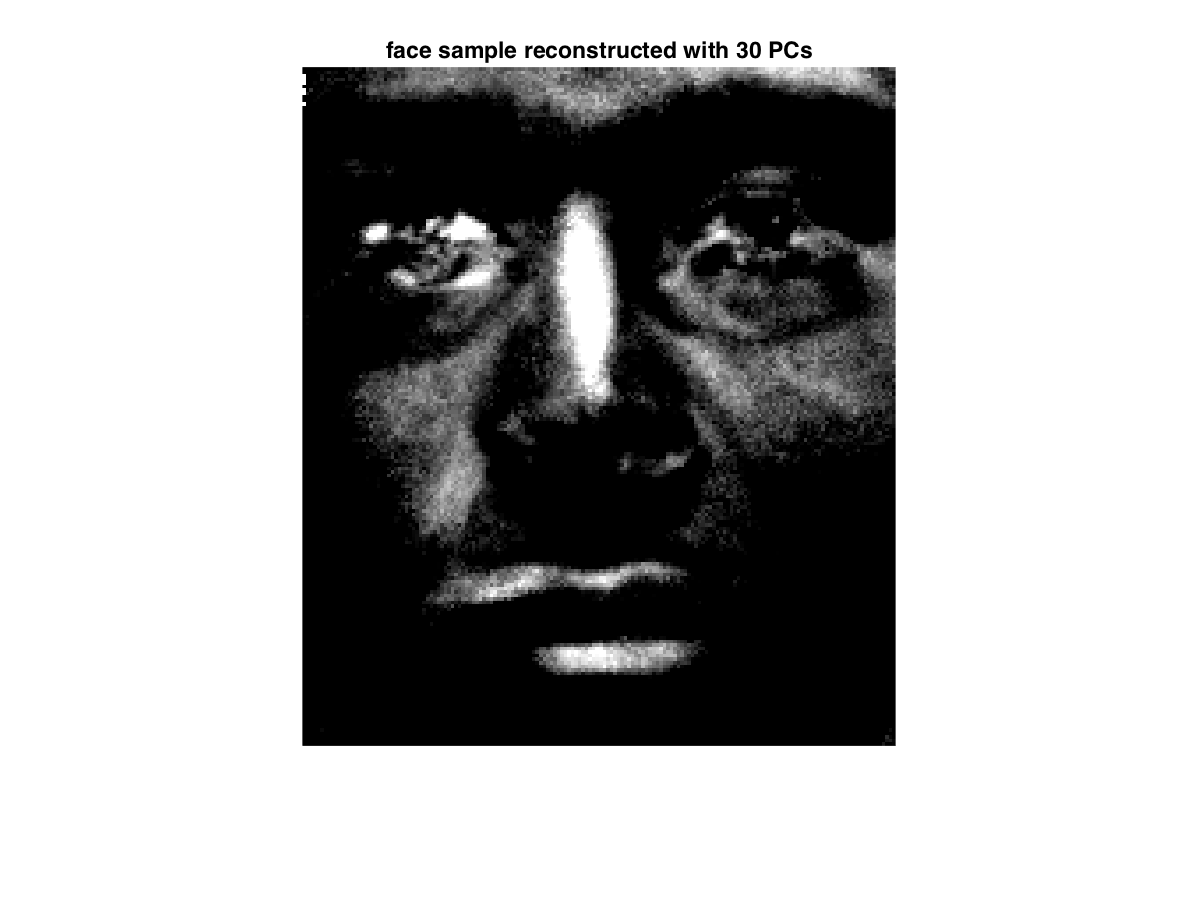
\includegraphics[width = 2in]{figures/SPM-Faces/face sample reconstructed with 30 PCs.png}} &
\subfloat[\fontsize{10}{11} IPCA ]{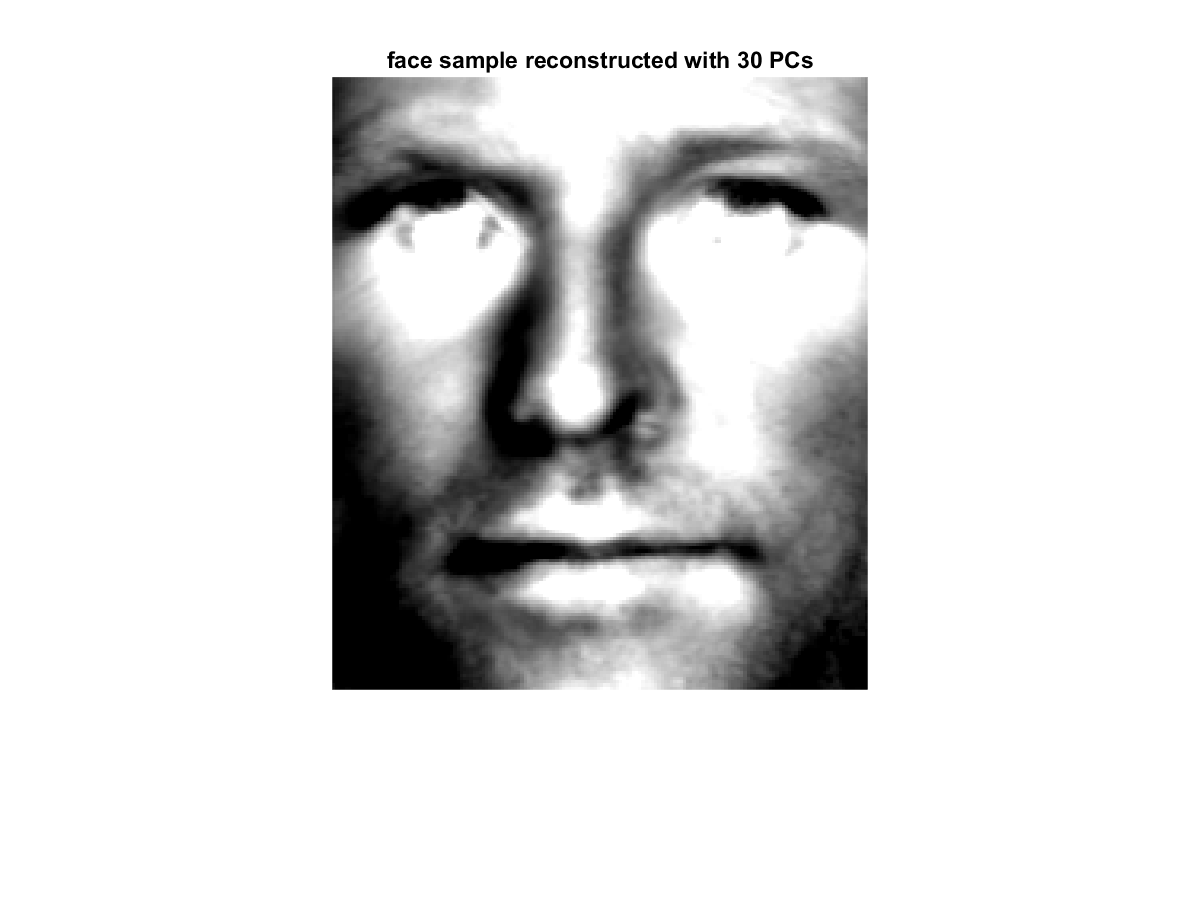
\includegraphics[width = 2in]{figures/IPCA-Faces/face sample reconstructed with 30 PCs.png}} \\
\subfloat[\fontsize{10}{11} MSG ]{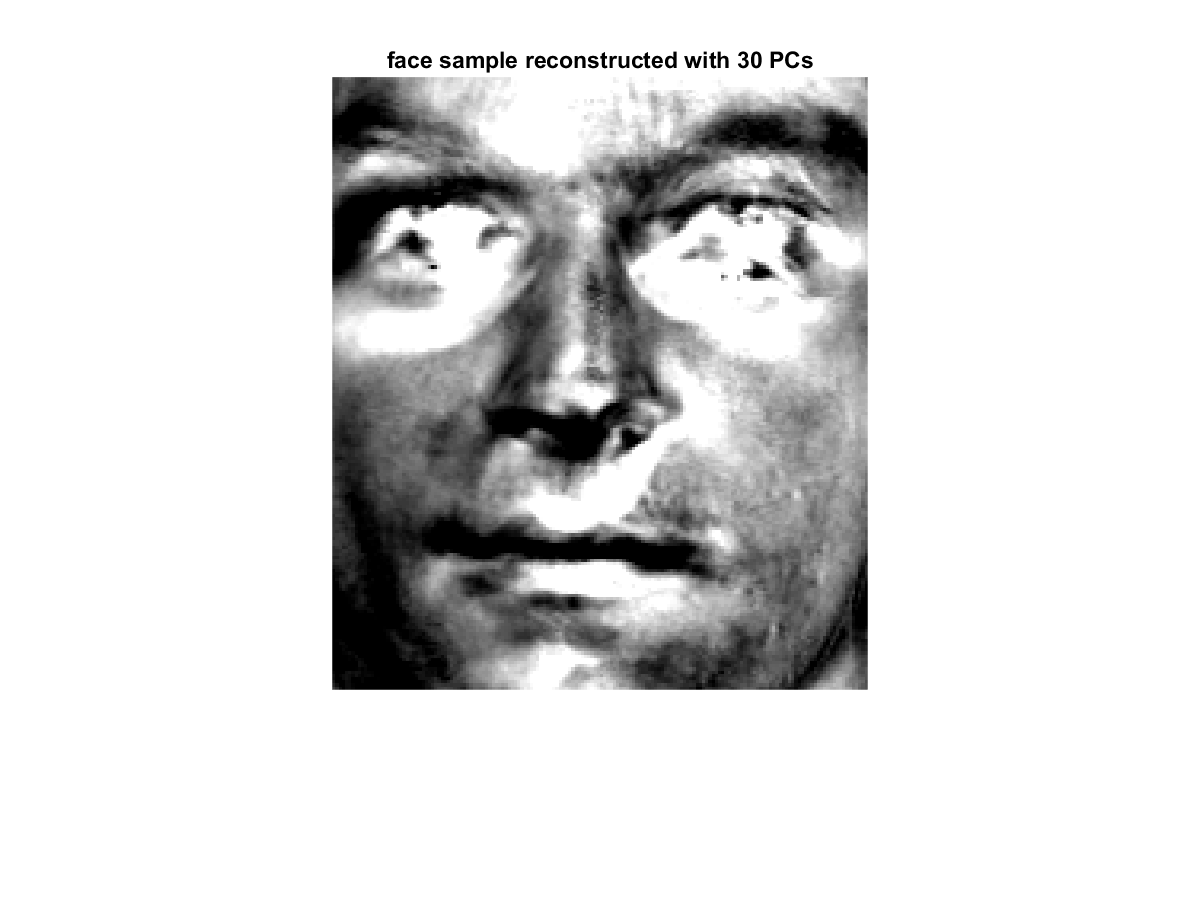
\includegraphics[width = 2in]{figures/MSG-Faces/face sample reconstructed with 30 PCs.png}} &
\subfloat[\fontsize{10}{11} SVD PCA ]{\includegraphics[width =2in]{figures/SVDPCA-Faces/face sample reconstructed with 30 PCs.png}} &
\subfloat[\fontsize{10}{11} SPCA ]{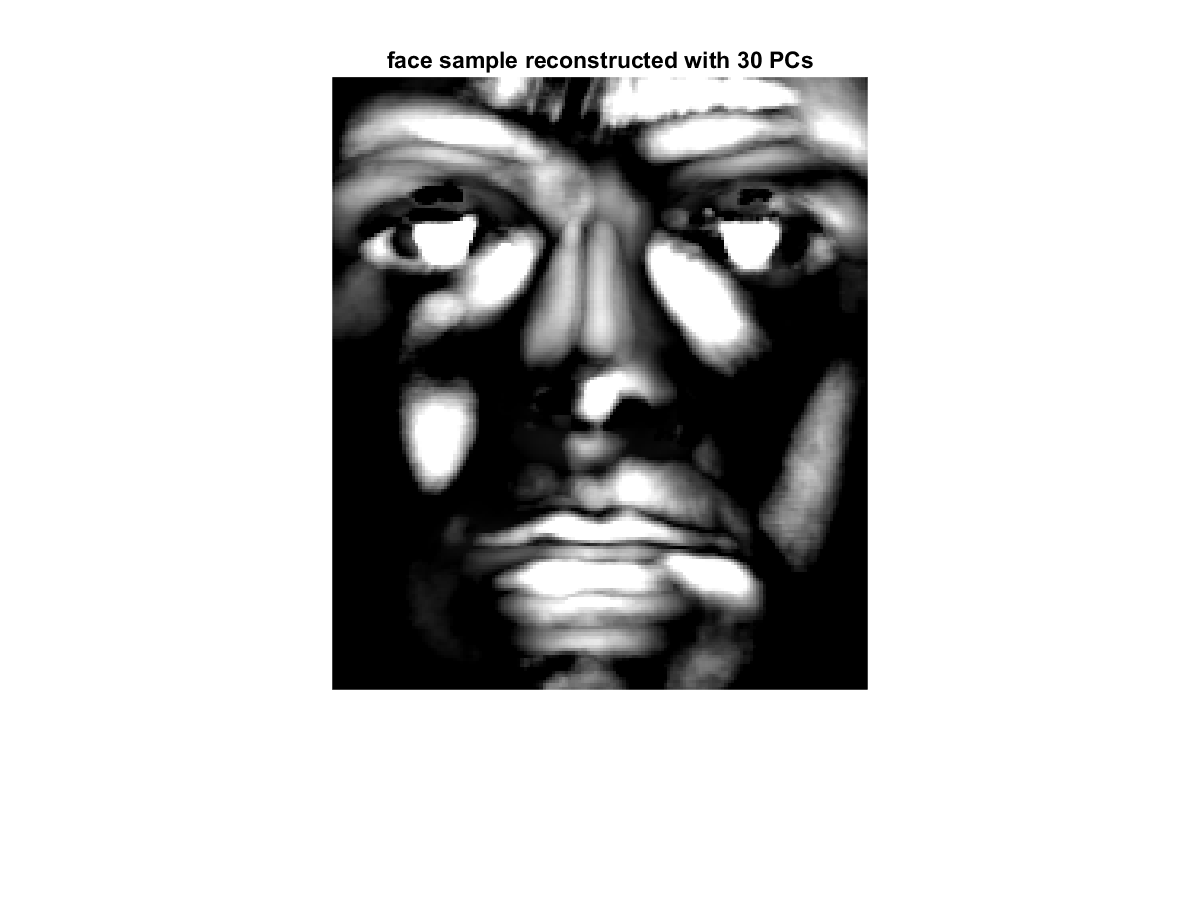
\includegraphics[width = 2in]{figures/SPCA-Faces/face sample reconstructed with 30 PCs.png}}  \\

\end{tabular}
\caption{\fontsize{10}{11} Reconstructed face with 30 Principle Components}
\end{figure*}


\begin{figure*}
\begin{tabular}{ccc}
\subfloat[\fontsize{10}{11}SVD PCA]{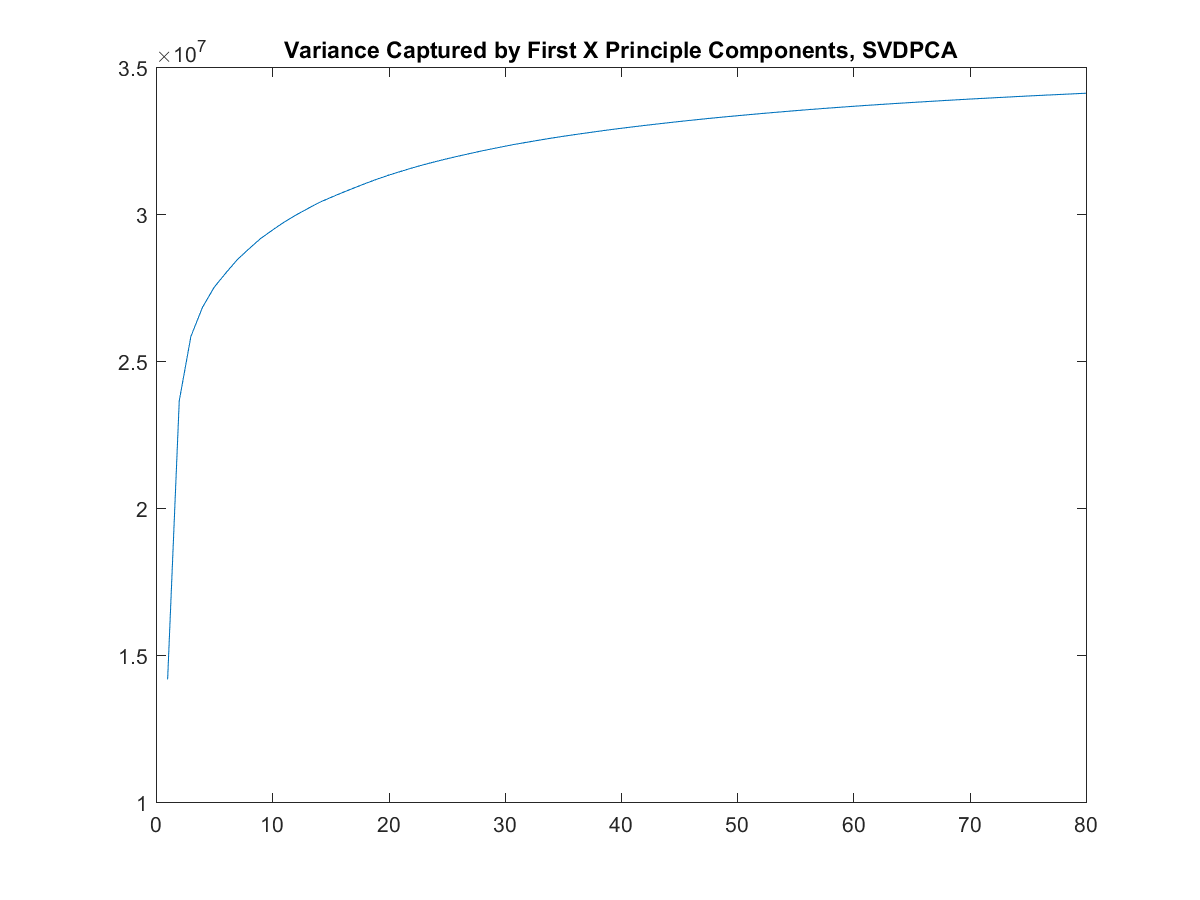
\includegraphics[width = 2in]{figures/Var SVDPCA.png}} &
\subfloat[\fontsize{10}{11}Stochastic Power Method]{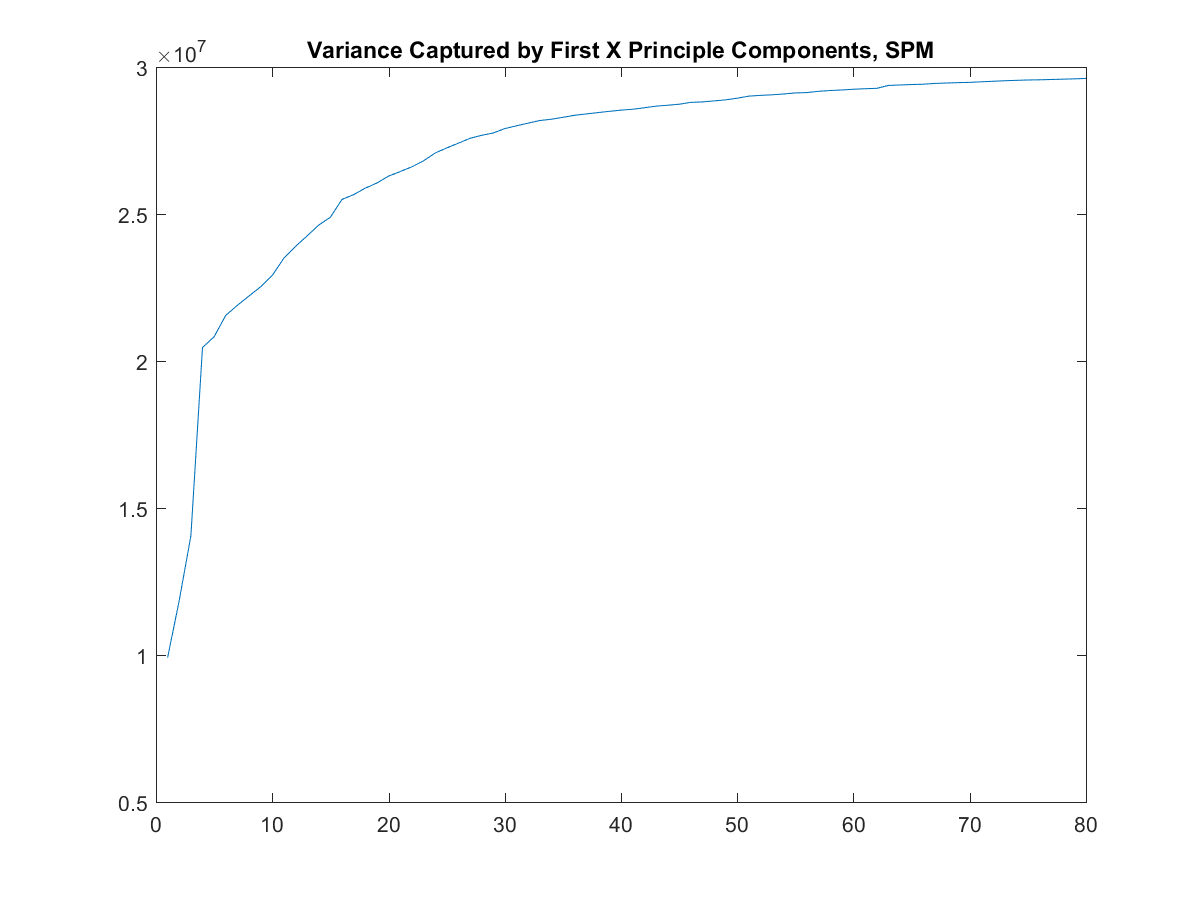
\includegraphics[width = 2in]{figures/Var SPM.png}} &
\subfloat[\fontsize{10}{11}Incremental PCA]{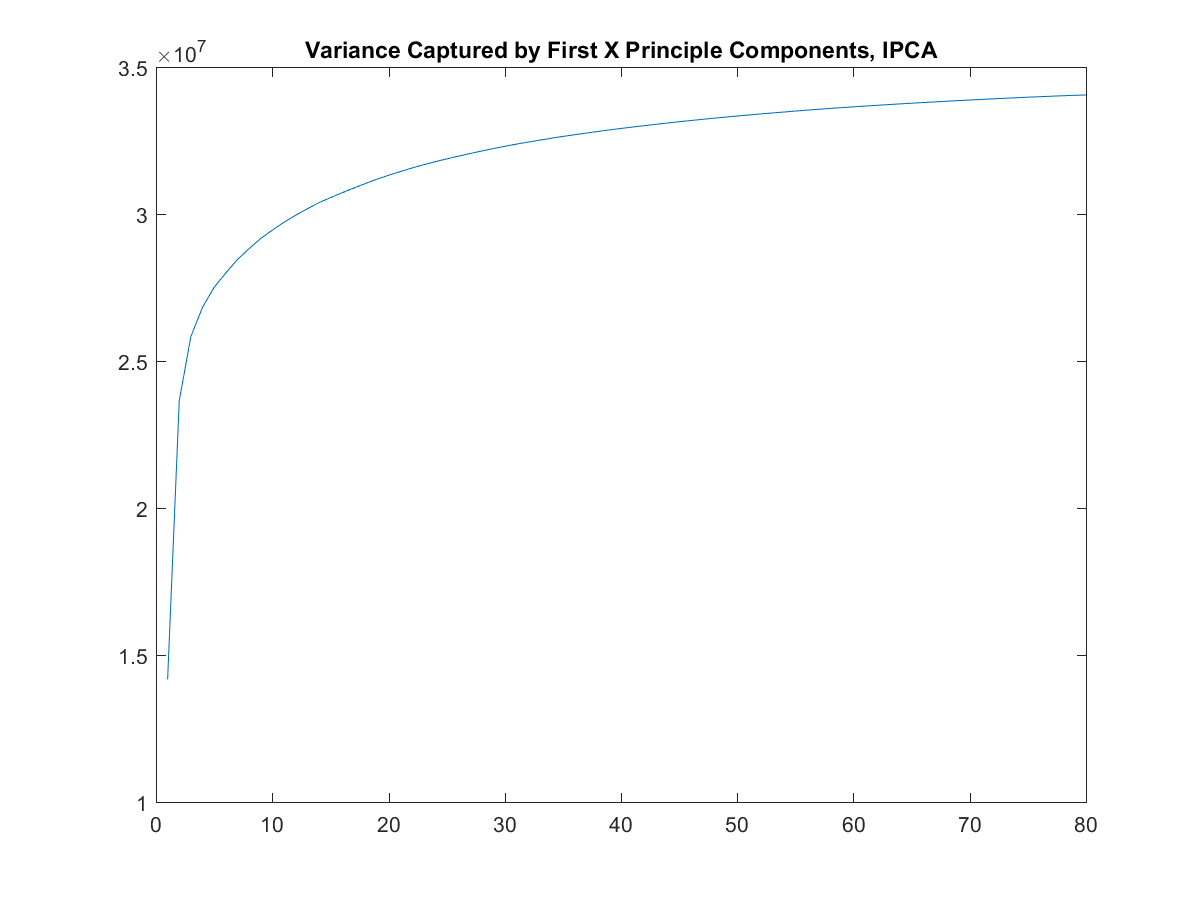
\includegraphics[width = 2in]{figures/Var IPCA.png}} \\
\subfloat[\fontsize{10}{11}Matrix Stochastic Gradient]{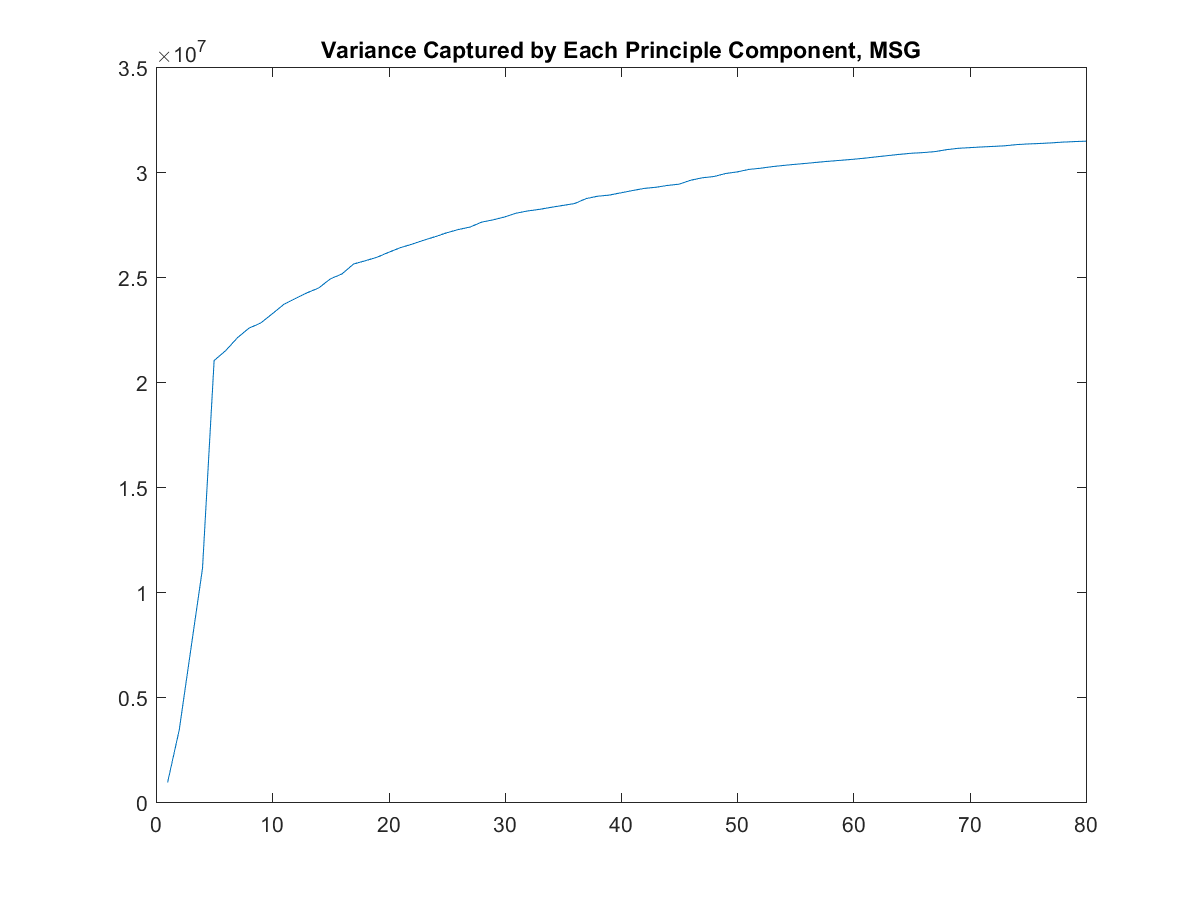
\includegraphics[width = 2in]{figures/Var MSG.png}} &
\subfloat[\fontsize{10}{11}Sparse PCA]{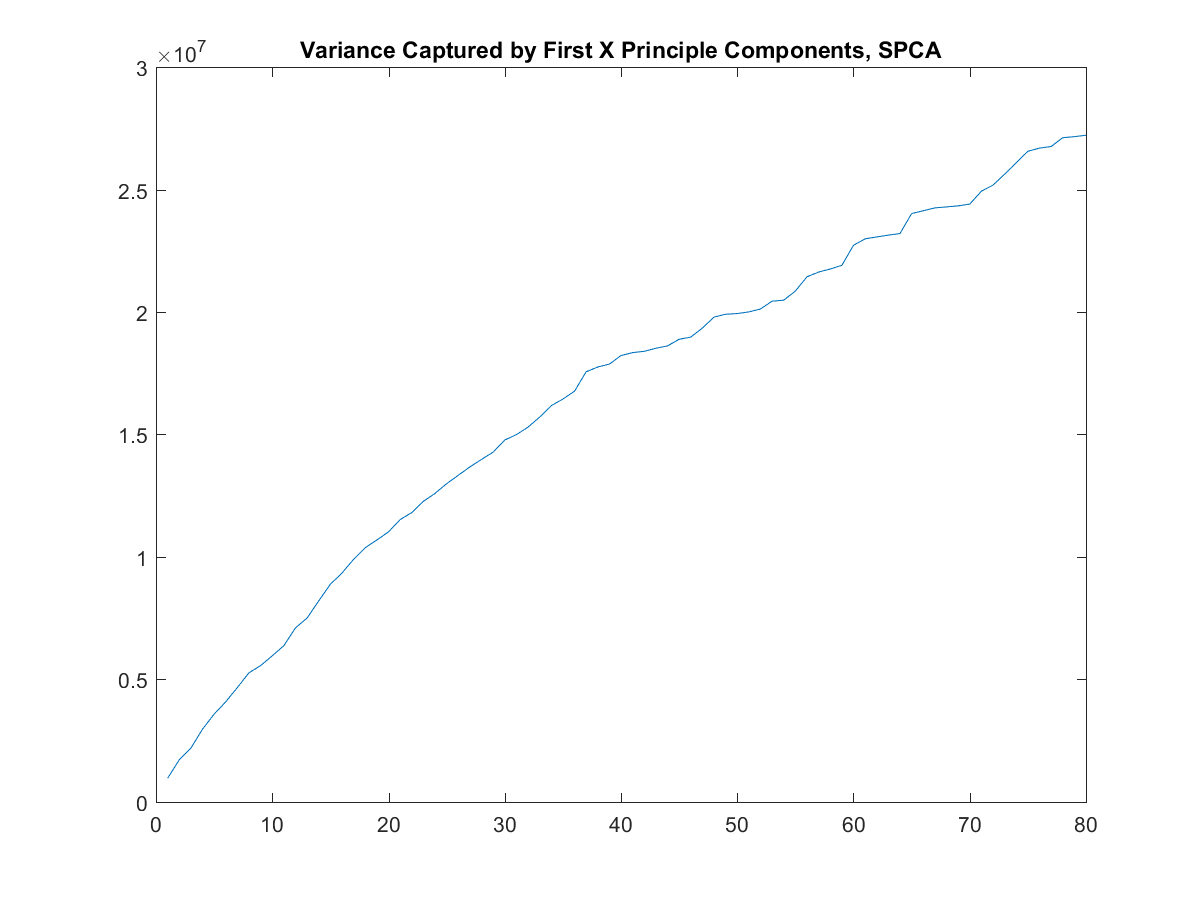
\includegraphics[width = 2in]{figures/Var SPCA.png}} 

\end{tabular}
\caption{\fontsize{10}{11} Variance Captured by Principle Components}
\end{figure*}




\section{Conclusion}

all algorithms for pca should learn the same subspace, up to small rotations and scalings...

discuss applications of streaming subspace learning

there are extensions for incremental kernal pca and dealing with the case of missing data...

\begin{thebibliography}{20}

%%cite these:

  \bibitem{achlioptas} 
  D. Achlioptas. Database-friendly random projections. In Proc. 20th Annu ACM SIGACT-SIGMOD-SIGART Symps. pages 274-281, 2001. 
  
  \bibitem{arora1} 
  Arora, R.; Cotter, A.; Livescu, K.; Srebro, N., "Stochastic optimization for PCA and PLS," in Communication, Control, and Computing (Allerton), 2012 50th Annual Allerton Conference on , vol., no., pp.861-868, 1-5 Oct. 2012
  
  \bibitem{Arora2}
   Arora, R., Cotter, A., and Srebro, N. 2013, arXiv:1307.1674 
  
  \bibitem{brand}  
  Brand, Matthew. {\em Incremental Singular Value Decomposition of Uncertain Data with Missing Values} In ECCV '02: Proceedings of the 7th European Conference on Computer Vision-Part I (2002), pp. 707-720
  
  \bibitem{clarkson}
  Clarkson, Kenneth L. "A randomized algorithm for closest-point queries." SIAM Journal on Computing 17.4 (1988): 830-847.
  
  \bibitem{engebretsen} 
  Engebretsen, L.; Indyk, P.; and O'Donnell, R. Derandomized dimensionality reductions with applications. In Proc. 13th Annu ACM-SIAM Sympos. Discrete Algor, 2002. 
  
    \bibitem{indyk} 
    P. Indyk. and R. Motwani. Approximate nearest neigbors: Towards removing the curse of dimsionality. In proc. 30th Annu. ACM Sympos. 2000.
  
  \bibitem{JL}  
  Johnson, W. B. and Lindenstrauss, J. Extensions of Lipschitz mappingsinto a Hilbert Space. Contemp. Math., 26:189-206, 1984.
  
  \bibitem{kushilevitz}
  Kushilevitz, Eyal, Rafail Ostrovsky, and Yuval Rabani. "Efficient search for approximate nearest neighbor in high dimensional spaces." SIAM Journal on Computing 30.2 (2000): 457-474.
 
  \bibitem{yale}  
 Lee, K. C; Ho, J. and Kriegman, D. "Acquiring Linear Subspaces for Face Recognition under Variable Lighting ", IEEE Trans. Pattern Anal. Mach. Intelligence 2005, volume 27 pgs 684-698.  
 
 \bibitem{turk}
 Turk, Matthew, and Alex Pentland. "Eigenfaces for recognition." Journal of cognitive neuroscience 3.1 (1991): 71-86.
  
  \bibitem{zou} 
  Zou, Hui, Trevor Hastie, and Robert Tibshirani. "Sparse principal component analysis." Journal of computational and graphical statistics 15.2 (2006): 265-286.
  
  \end{thebibliography}




\end{document}
